\documentclass{article}
\usepackage{booktabs}
%\usepackage{ctex}
\usepackage{fancyhdr}
\usepackage{extramarks}
\usepackage{amsmath}
\usepackage{amsthm}
\usepackage{amsfonts}
\usepackage{tikz}
\usepackage[plain]{algorithm}
\usepackage{algpseudocode}
\usepackage{extarrows}
\usepackage{indentfirst}

\usepackage[titletoc]{appendix}
\usepackage{pythonhighlight}
\usepackage{listings}
\usepackage[framed,numbered,autolinebreaks,useliterate]{mcode}

\usetikzlibrary{automata,positioning}

%
% Basic Document Settings
%

\topmargin=-0.45in
\evensidemargin=0in
\oddsidemargin=0in
\textwidth=6.5in
\textheight=9.0in
\headsep=0.25in

\linespread{1.1}

\pagestyle{fancy}
\lhead{\hmwkAuthorName}
\chead{\hmwkClass\ : \hmwkTitle}
\rhead{}
\lfoot{\lastxmark}
\cfoot{\thepage}

\renewcommand\headrulewidth{0.4pt}
\renewcommand\footrulewidth{0.4pt}

\setlength\parindent{2em}

%
% Create Problem Sections
%



\setcounter{secnumdepth}{0}
\newcounter{partCounter}
\newcounter{homeworkProblemCounter}
\setcounter{homeworkProblemCounter}{1}
\nobreak\extramarks{Problem \arabic{homeworkProblemCounter}}{}\nobreak{}

%
% Homework Problem Environment
%
% This environment takes an optional argument. When given, it will adjust the
% problem counter. This is useful for when the problems given for your
% assignment aren't sequential. See the last 3 problems of this template for an
% example.
%


%
% Homework Details
%   - Title
%   - Due date
%   - Class
%   - Section/Time
%   - Instructor
%   - Author
%

\newcommand{\hmwkTitle}{Initial Problems for ODE}
\newcommand{\hmwkDueDate}{May, 2022}
\newcommand{\hmwkClass}{Chap 5}
\newcommand{\hmwkClassTime}{}
\newcommand{\hmwkClassInstructor}{}
\newcommand{\hmwkAuthorName}{\textbf{Yuchen Ge}}

%
% Title Page
%

\title{
    \vspace{2in}
    \textmd{\textbf{\hmwkClass:\ \hmwkTitle}}\\
    \normalsize\vspace{0.1in}\small{Due\ on\ \hmwkDueDate\ }\\
    \vspace{0.1in}\large{\textit{\hmwkClassInstructor\ \hmwkClassTime}}
    \vspace{3in}
}

\author{\hmwkAuthorName}
\date{}

\renewcommand{\part}[1]{\textbf{\large Part \Alph{partCounter}}\stepcounter{partCounter}\\}

%
% Various Helper Commands
%

% Useful for algorithms
\newcommand{\alg}[1]{\textsc{\bfseries \footnotesize #1}}

% For derivatives
\newcommand{\deriv}[1]{\frac{\mathrm{d}}{\mathrm{d}x} (#1)}

% For partial derivatives
\newcommand{\pderiv}[2]{\frac{\partial}{\partial #1} (#2)}

% Integral dx
\newcommand{\dx}{\mathrm{d}x}

% Alias for the Solution section header
\newcommand{\solution}{\textbf{\large Solution}}

% Probability commands: Expectation, Variance, Covariance, Bias
\newcommand{\C}{\mathrm{C}}
\newcommand{\D}{\mathrm{D}}
\newcommand{\E}{\mathrm{E}}
\newcommand{\U}{\mathrm{U}}
\newcommand{\Z}{\mathbb{Z}}
\newcommand{\R}{\mathbb{R}}
\newcommand{\Q}{\mathbb{Q}}
\newcommand{\N}{\mathbb{N}}
\begin{document}
\maketitle

\pagebreak
\section{1. Introduction}

The chapter mianly deals with the problem of initial problems for ODE.

First we claim that all function and variable names are self-clear. And a/b is interpreted to be section a question b, e.g. 5.4/7.

\section{2. Application of Eular's Method (5.2/7)}

\subsection{2.1 Program Running and Data Analysis }
    
    Question 5.2/7 a. requires the best approximation of the initial problem. First we calculate the real value 
    $$ y(5)=e^{-5}+5=5.006737946999086.
    $$
    Then we apply Eular's Method with parameters $h=0.2,0.1,0.05$. We run the program as follows. (Meanwhile we display the running time.)
    \begin{figure}[h]
    \centering
    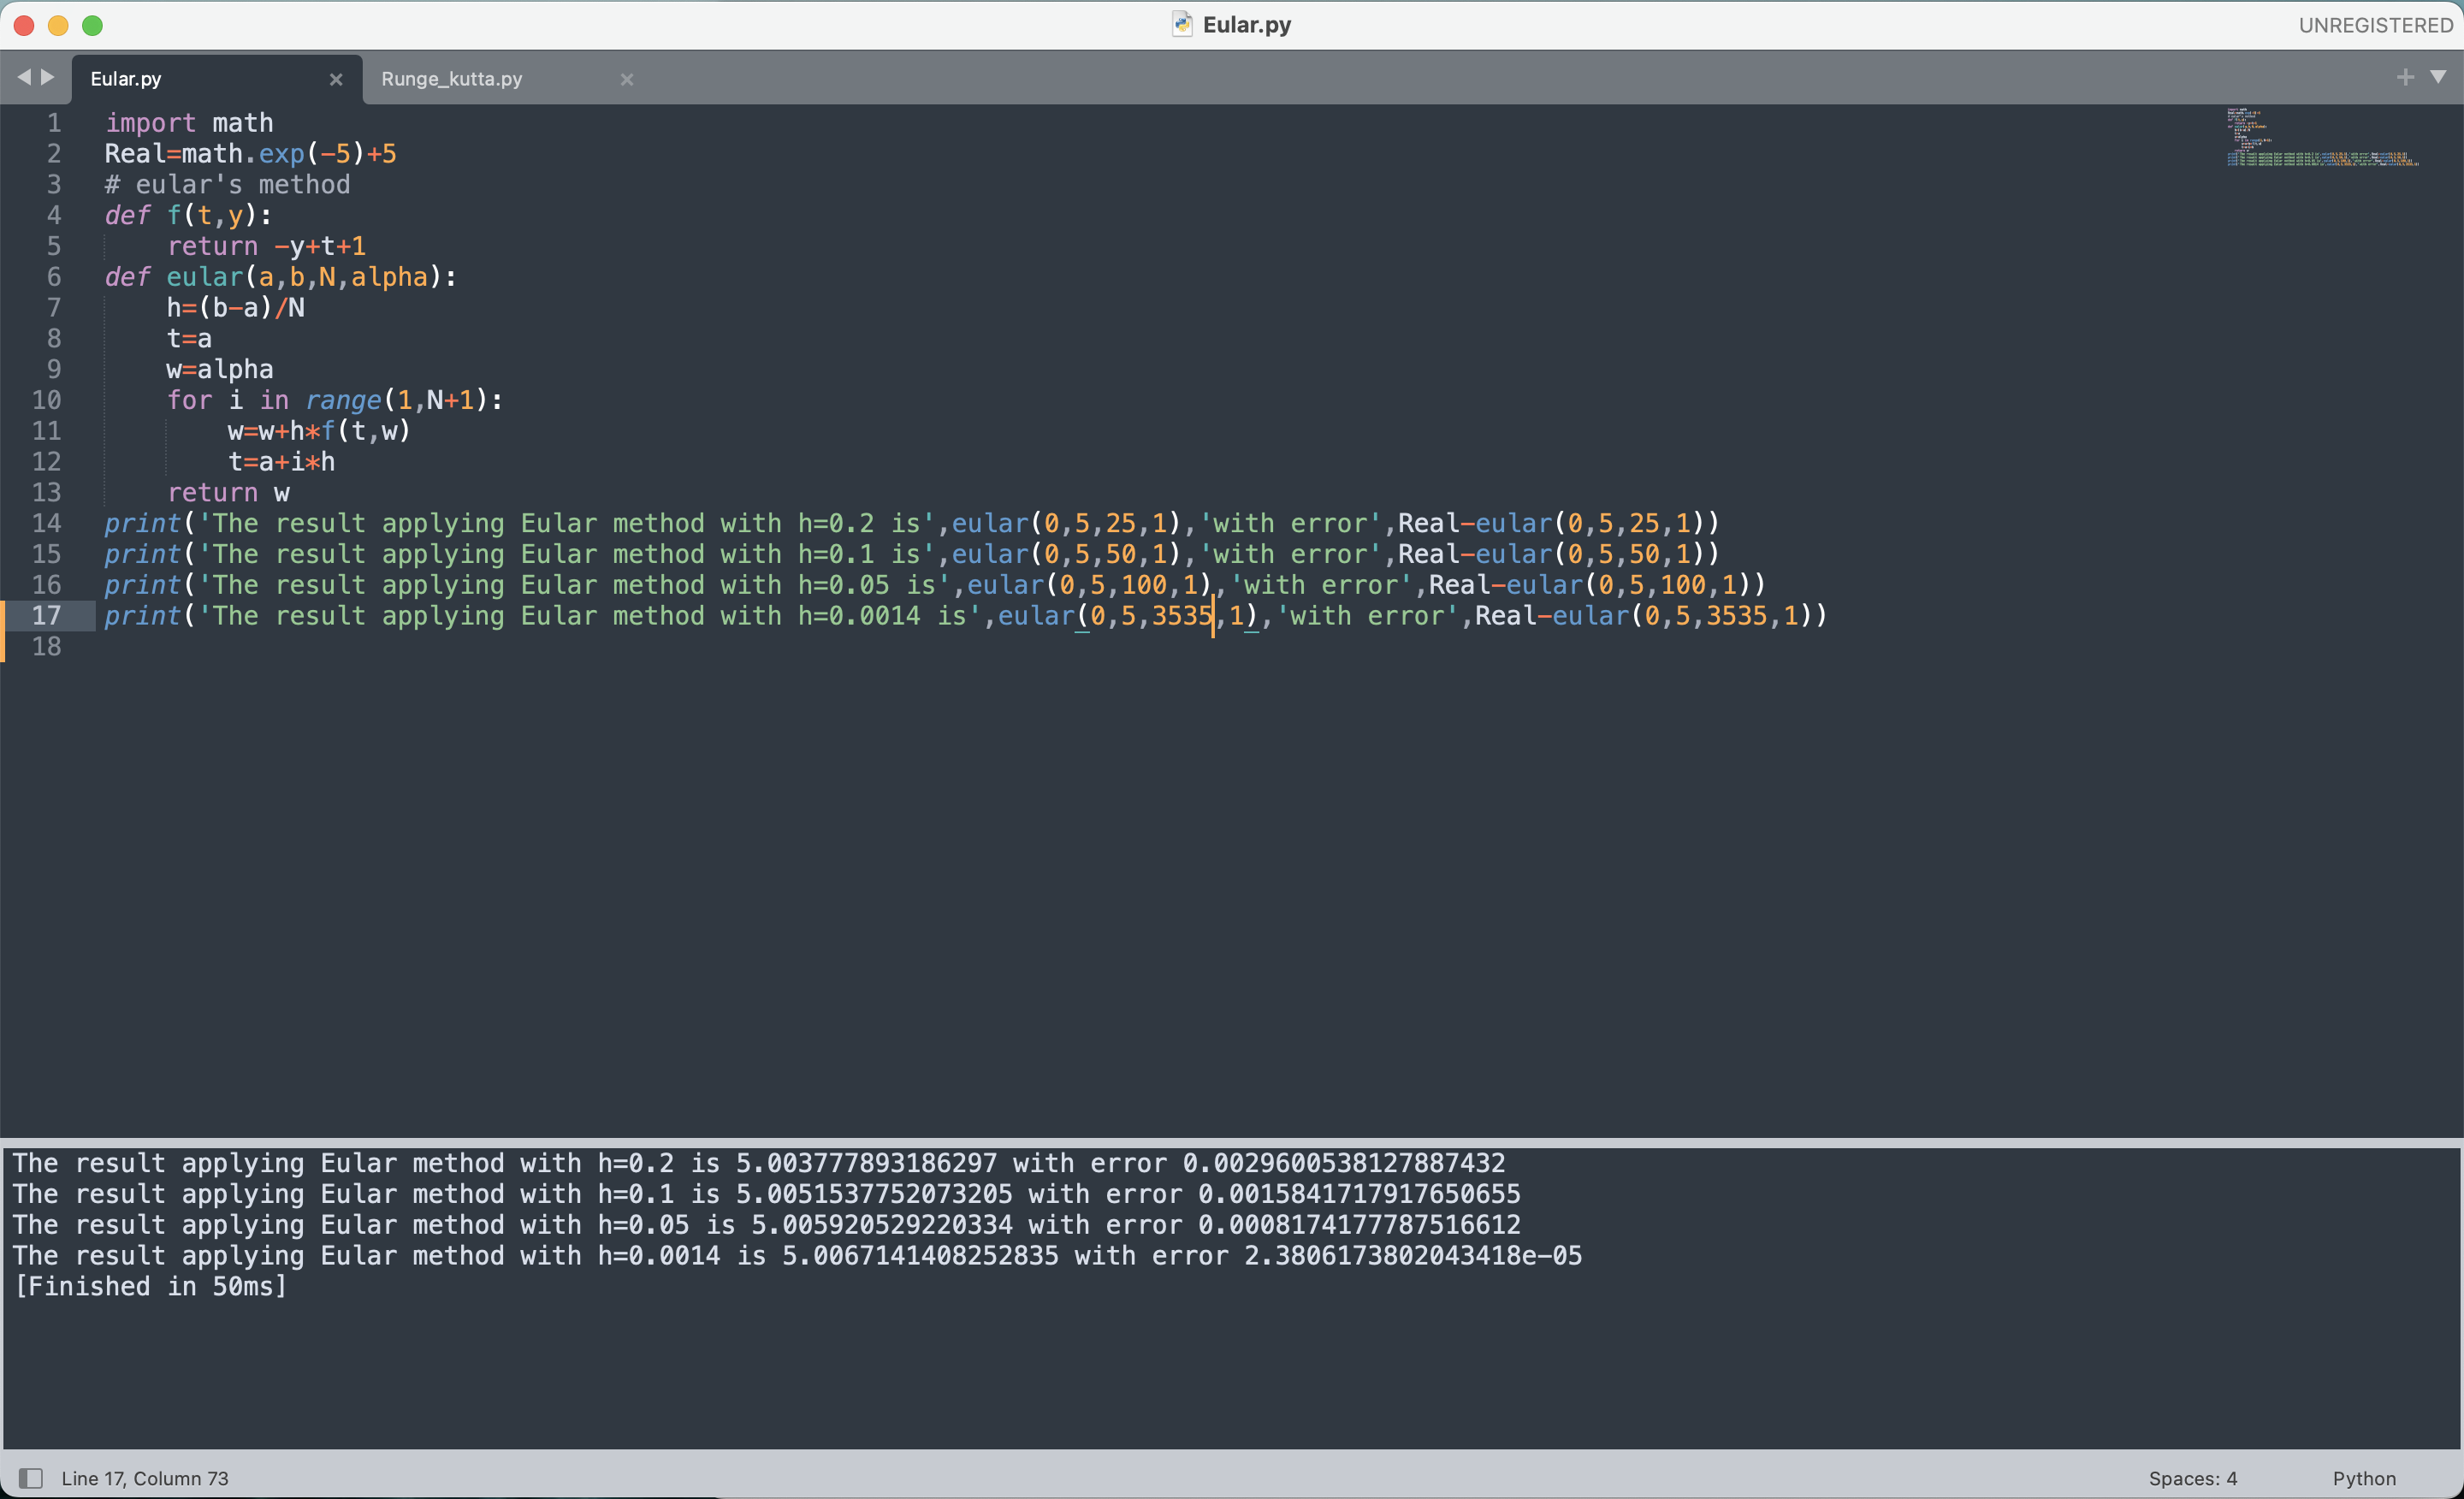
\includegraphics[scale=0.25]{Program1}
    \end{figure}

    We write down the results in the table below, where we \textbf{reserve seven significant digits} for the result.
    \begin{table}[htbp]
    \centering
    \caption{Results of 5.2/7}
    \begin{tabular}{c|c|c}
    \toprule
     h & \textbf{Approximation of y(5)} & \textbf{Error} \\ 
    \midrule
    0.2 & 5.003778 & 0.002960 \\
    0.1 & 5.005154 & 0.001584 \\
    0.05 & 5.005921 & 0.000817 \\
    \bottomrule
    \end{tabular}
    \end{table}

    For question 5.2/7 b., we apply formula (5.14)
    $$ h=\sqrt{\frac{2\delta}{M}}=(\frac{2\cdot 10^{-6}}{1})^{1/2}=0.001414213562373095\approx0.0014142.
    $$

    Then we run the program as above and we have the approximation of $y(5)\approx 5.00671414.$

\section{3. Application of Runge-Kutta's Method (5.4/4c,5c,6,7,8,9,11,12)}
    \subsection{3.1 Program Running and Data Analysis of 5.4/4c,5c} 
    Applying Modified Eular's method for $y'=-(y+1)(y+3)$ with initial value $y(0)=-2$ (5.4/4c), we run the program as follows: (Meanwhile we also display the running time as a byproduct.)
    \begin{figure}[h]
    \centering
    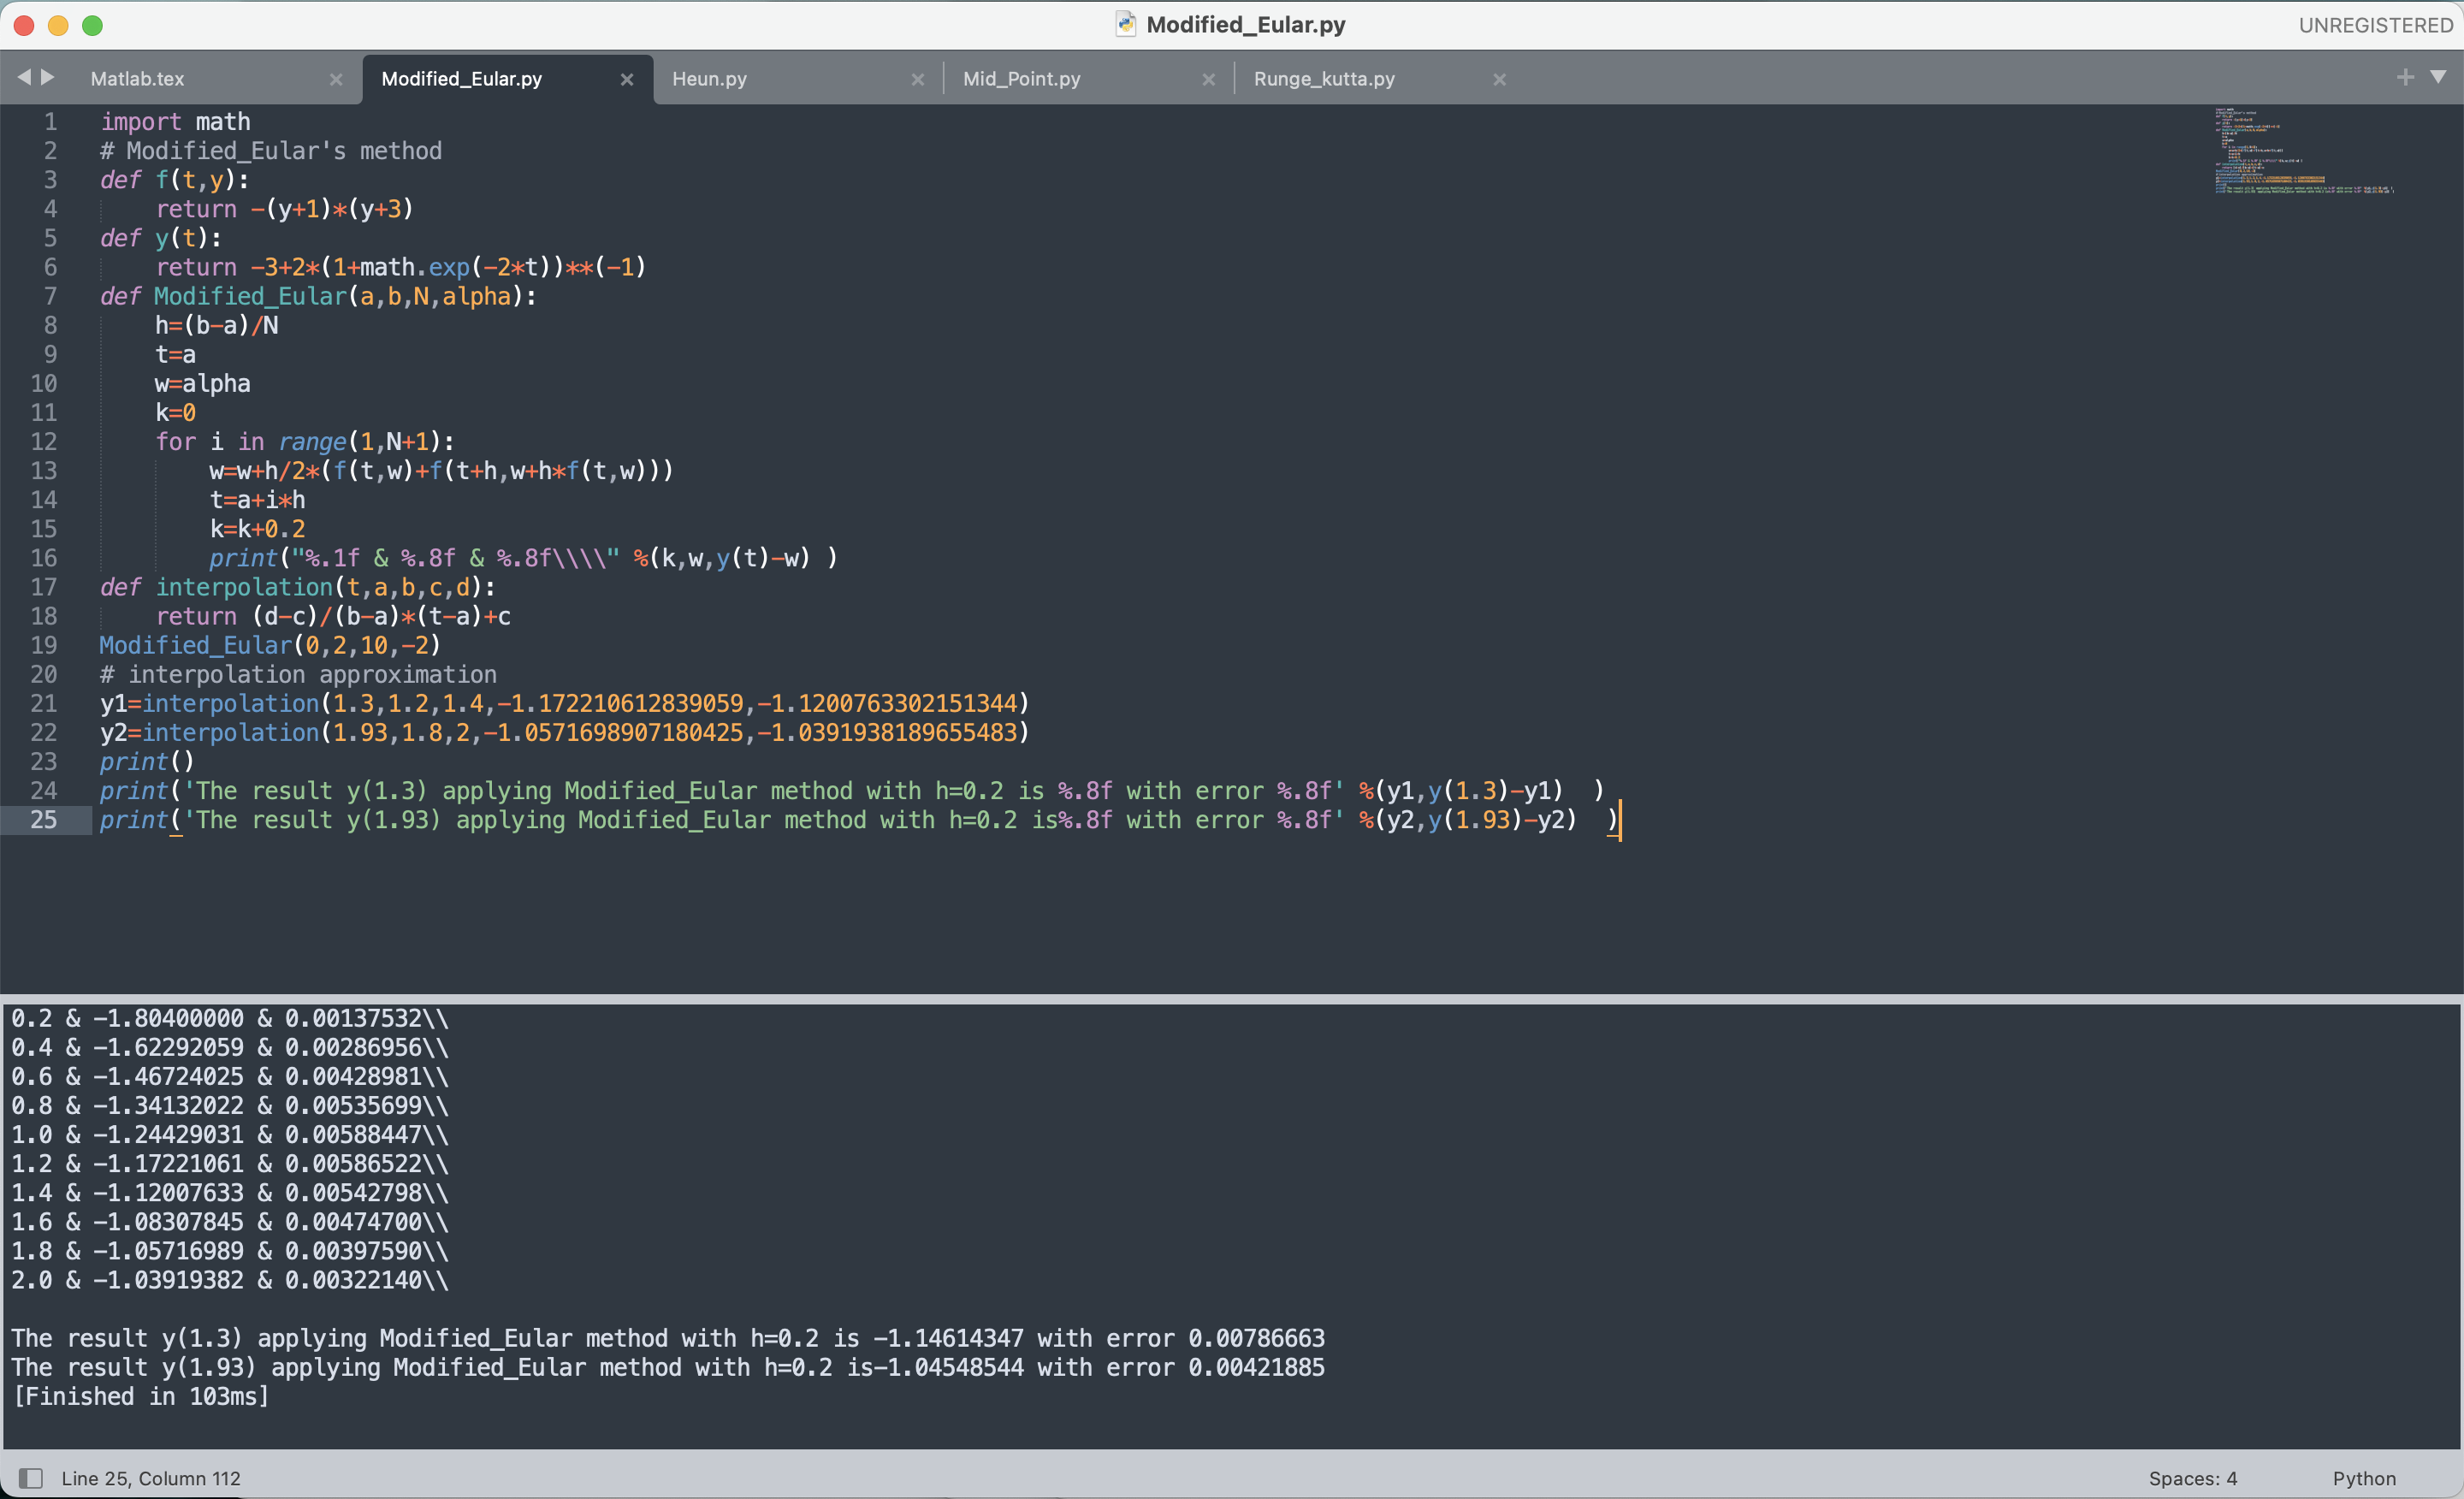
\includegraphics[scale=0.25]{Program2}
    \end{figure}

    And therefore we give a table containing results and errors: (reserve nine significant digits)
    \begin{table}[htbp]
    \centering
    \caption{Results of 5.4/4c (Modified Eular's method)}
    \begin{tabular}{c|c|c}
    \toprule
    t& \textbf{Approximation of y(t)} & \textbf{Error} \\ 
    \midrule
    0.2 & -1.80400000 & 0.00137532\\
    0.4 & -1.62292059 & 0.00286956\\
    0.6 & -1.46724025 & 0.00428981\\
    0.8 & -1.34132022 & 0.00535699\\
    1.0 & -1.24429031 & 0.00588447\\
    1.2 & -1.17221061 & 0.00586522\\
    1.4 & -1.12007633 & 0.00542798\\
    1.6 & -1.08307845 & 0.00474700\\
    1.8 & -1.05716989 & 0.00397590\\
    2.0 & -1.03919382 & 0.00322140\\
    \bottomrule
    \end{tabular}
    \end{table}

    And we find that the error term grows until $t=1.2$, which is contractdict to the earlier claim for Eular's method that the error monotonically increases with t increases. The reason behind this is that Eular's method requires only the term $f(t_i,w_i)$, while the other methods like the Modified Eular Method requires terms below which is much more comlicated,
    $$ \frac{h}{2}[f(t_{i},w_{i})+f(t_{i+1},w_{i}+hf(t_i,w_i))].
    $$

    Then for  5.4/5c we use the approximation value of $y(1.2)$ and $y(1.4)$ to linear interpolate $y(1.3)$, which leads to 
    $$ \tilde{y}(1.3)=\frac{\tilde{y}(1.4)-\tilde{y}(1.2)}{1.4-1.2}(1.3-1.2)+\tilde{y}(1.2)=-1.1461434715270966
    $$
    where we denote the approximation value of $y(1.3)$ by $\tilde{y}(1.3)$.
    Similarly, we have $\tilde{y}(1.93)=-1.0454854440789212$. And thus gather the information for the table ( reserve nine significant digits ):
    \begin{table}[htbp]
    \centering
    \caption{Results of 5.4/5c (Modified Eular's method)}
    \begin{tabular}{c|c|c}
    \toprule
    t& \textbf{Approximation of y(t)} & \textbf{Error} \\ 
    \midrule
    1.3 & -1.14614347 & 0.00786663 \\
    1.93 & -1.04548544 & 0.00421885 \\
    \bottomrule
    \end{tabular}
    \end{table}

\subsection{3.2 Program Running and Data Analysis of 5.4/6,7} 

    Similarly we apply Heun method and run the program as follows:

    \begin{figure}[h]
    \centering
    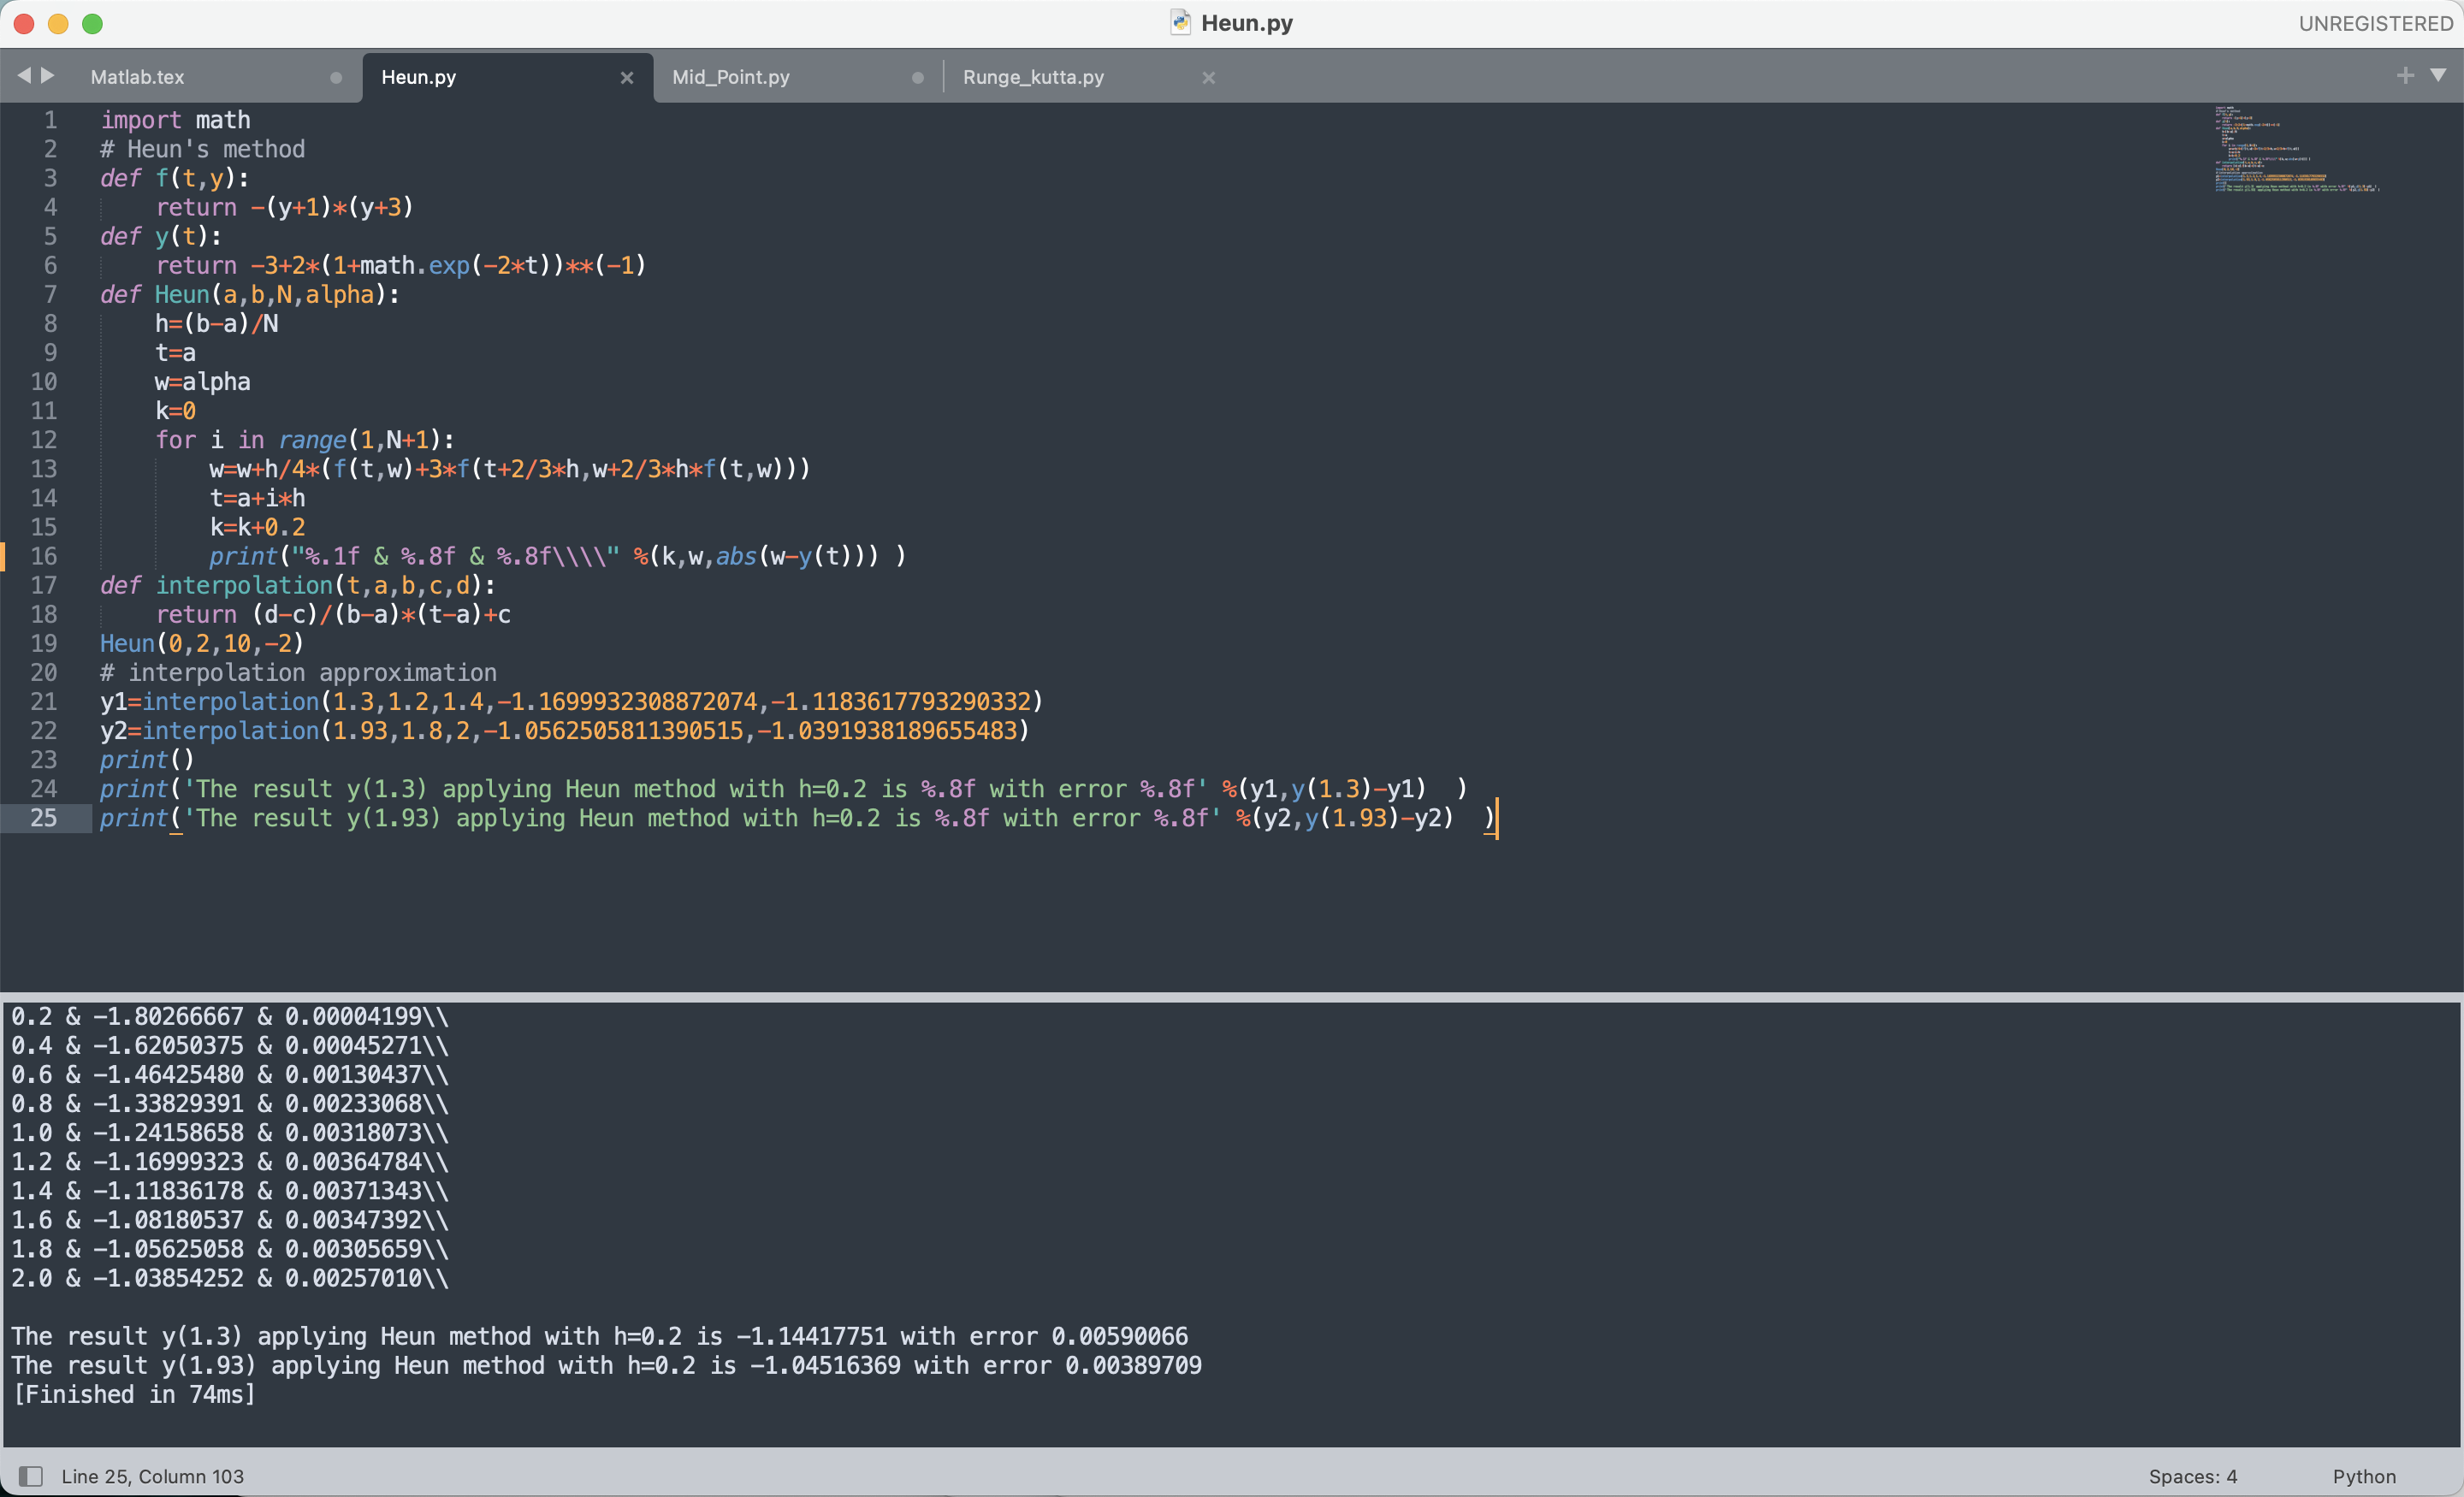
\includegraphics[scale=0.22]{Program3}
    \end{figure}

    And therefore we can give a table containing results and errors, where we reserve nine significant digits for the results.

    \begin{table}[htbp]
    \centering
    \caption{Results of 5.4/6 (Heun method)}
    \begin{tabular}{c|c|c}
    \toprule
    t& \textbf{Approximation of y(t)} & \textbf{Error} \\ 
    \midrule
    0.2 & -1.80266667 & 0.00004199\\
    0.4 & -1.62050375 & 0.00045271\\
    0.6 & -1.46425480 & 0.00130437\\
    0.8 & -1.33829391 & 0.00233068\\
    1.0 & -1.24158658 & 0.00318073\\
    1.2 & -1.16999323 & 0.00364784\\
    1.4 & -1.11836178 & 0.00371343\\
    1.6 & -1.08180537 & 0.00347392\\
    1.8 & -1.05625058 & 0.00305659\\
    2.0 & -1.03854252 & 0.00257010\\
    \bottomrule
    \end{tabular}
    \end{table}

    Also we find that the error term grows until $t=1.6$, which is contractdict to the earlier claim for Eular's method that the error monotonically increases with t increases. The reason behind this is the same.

    Then for  5.4/7, similarly, we can interpolate in the same way as above and thus gives the table (reserve nine significant digits):
    \begin{table}[htbp]
    \centering
    \caption{Results of 5.4/7 (Heun method)}
    \begin{tabular}{c|c|c}
    \toprule
    t& \textbf{Approximation of y(t)} & \textbf{Error} \\ 
    \midrule
    1.3 & -1.14417751 & 0.00590066 \\
    1.93 & -1.04516369 & 0.00389709 \\
    \bottomrule
    \end{tabular}
    \end{table}

\subsection{3.3 Program Running and Data Analysis of 5.4/8,9} 
    Similarly we apply Midpoint method and run the program as follows:

    \begin{figure}[h]
    \centering
    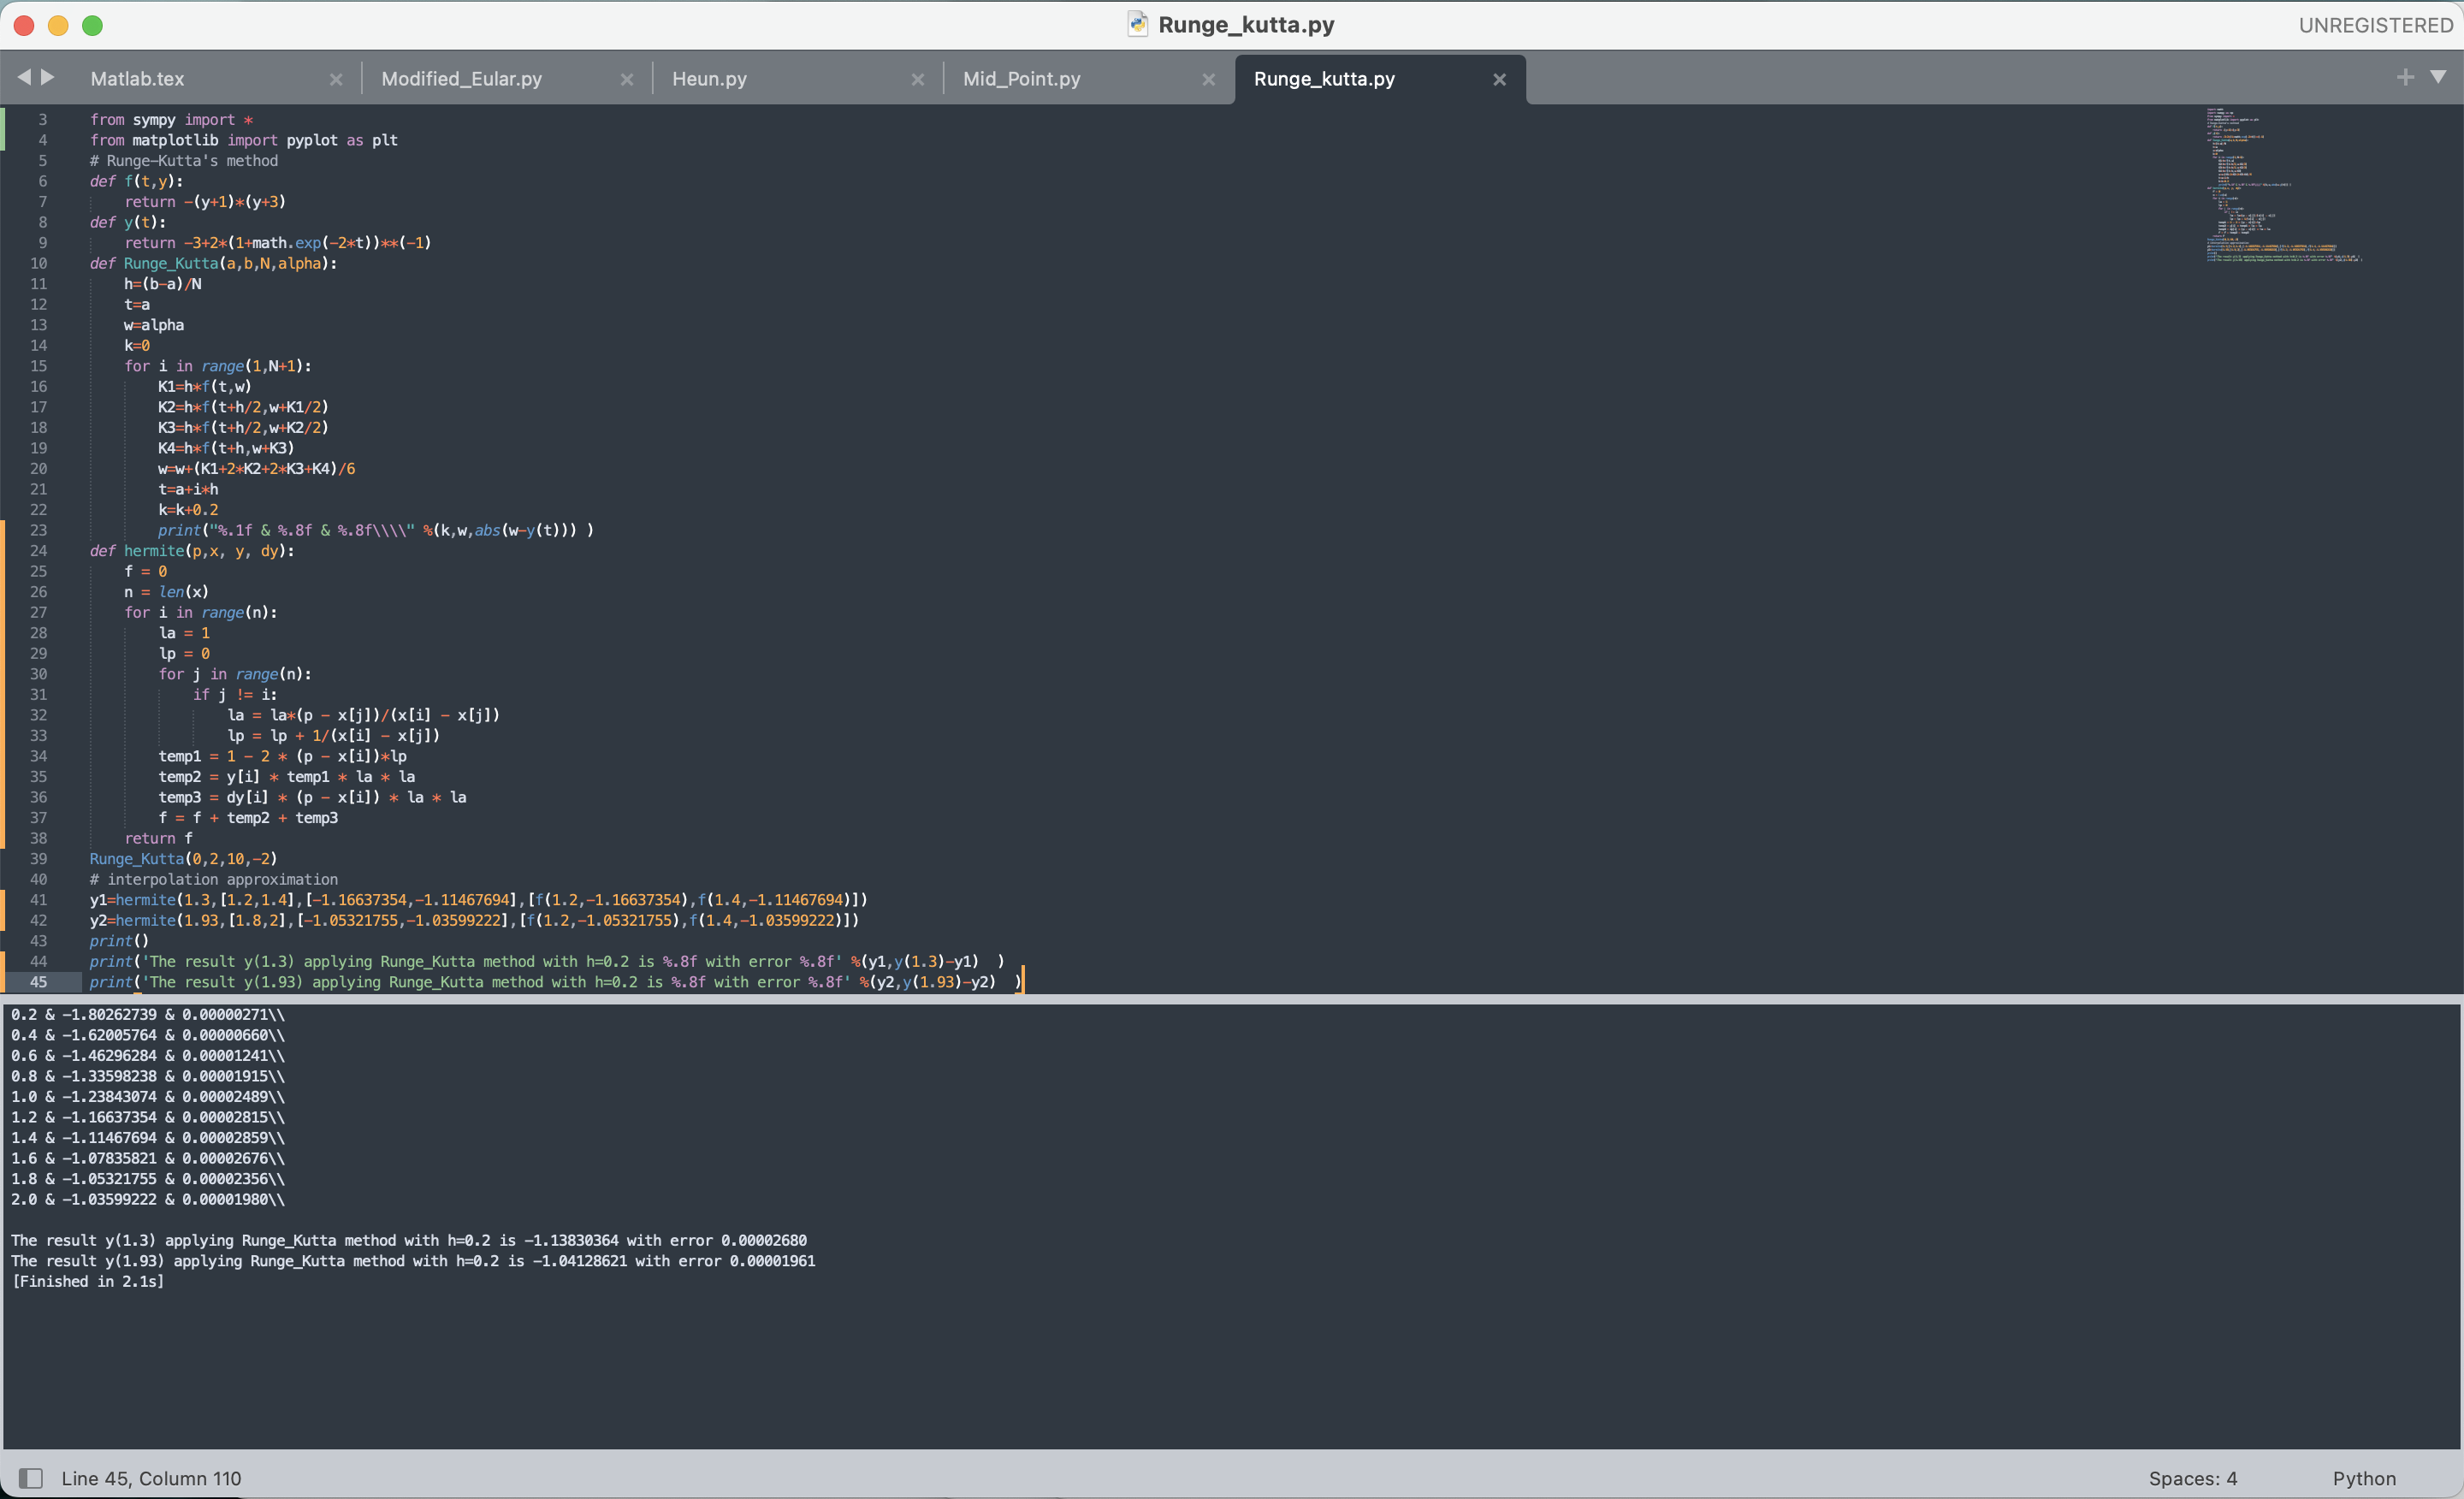
\includegraphics[scale=0.22]{Program4}
    \end{figure}

    And therefore we give a table containing results and errors. 

    \begin{table}[htbp]
    \centering
    \caption{Results of 5.4/8 (Midpoint method)}
    \begin{tabular}{c|c|c}
    \toprule
    t& \textbf{Approximation of y(t)} & \textbf{Error} \\ 
    \midrule
    0.2 & -1.80200000 & 0.00062468\\
    0.4 & -1.61929656 & 0.00075448\\
    0.6 & -1.46276690 & 0.00018353\\
    0.8 & -1.33678999 & 0.00082676\\
    1.0 & -1.24024699 & 0.00184114\\
    1.2 & -1.16889759 & 0.00255219\\
    1.4 & -1.11751649 & 0.00286814\\
    1.6 & -1.08117882 & 0.00284737\\
    1.8 & -1.05579872 & 0.00260473\\
    2.0 & -1.03822270 & 0.00225028\\
    \bottomrule
    \end{tabular}
    \end{table}

    Also we find that the error term grows until $t=1.6$, which is contractdict to the earlier claim for Eular's method that the error monotonically increases with t increases. The reason behind this is the same.

    Then for  5.4/9 , similarly, we can interpolate in the same way as above and thus gives the table (reserve nine significant digits):
    \begin{table}[htbp]
    \centering
    \caption{Results of 5.4/9 (Midpoint method)}
    \begin{tabular}{c|c|c}
    \toprule
    t& \textbf{Approximation of y(t)} & \textbf{Error} \\ 
    \midrule
    1.3 & -1.14320704 & 0.00493020 \\
    1.93 & -1.04437431 & 0.00310771 \\
    \bottomrule
    \end{tabular}
    \end{table}

\newpage
\subsection{3.4 Program Running and Data Analysis of 5.4/11,12} 
    And similarly we apply Runge-Kutta's method method and run the program as follows:

    \begin{figure}[h]
    \centering
    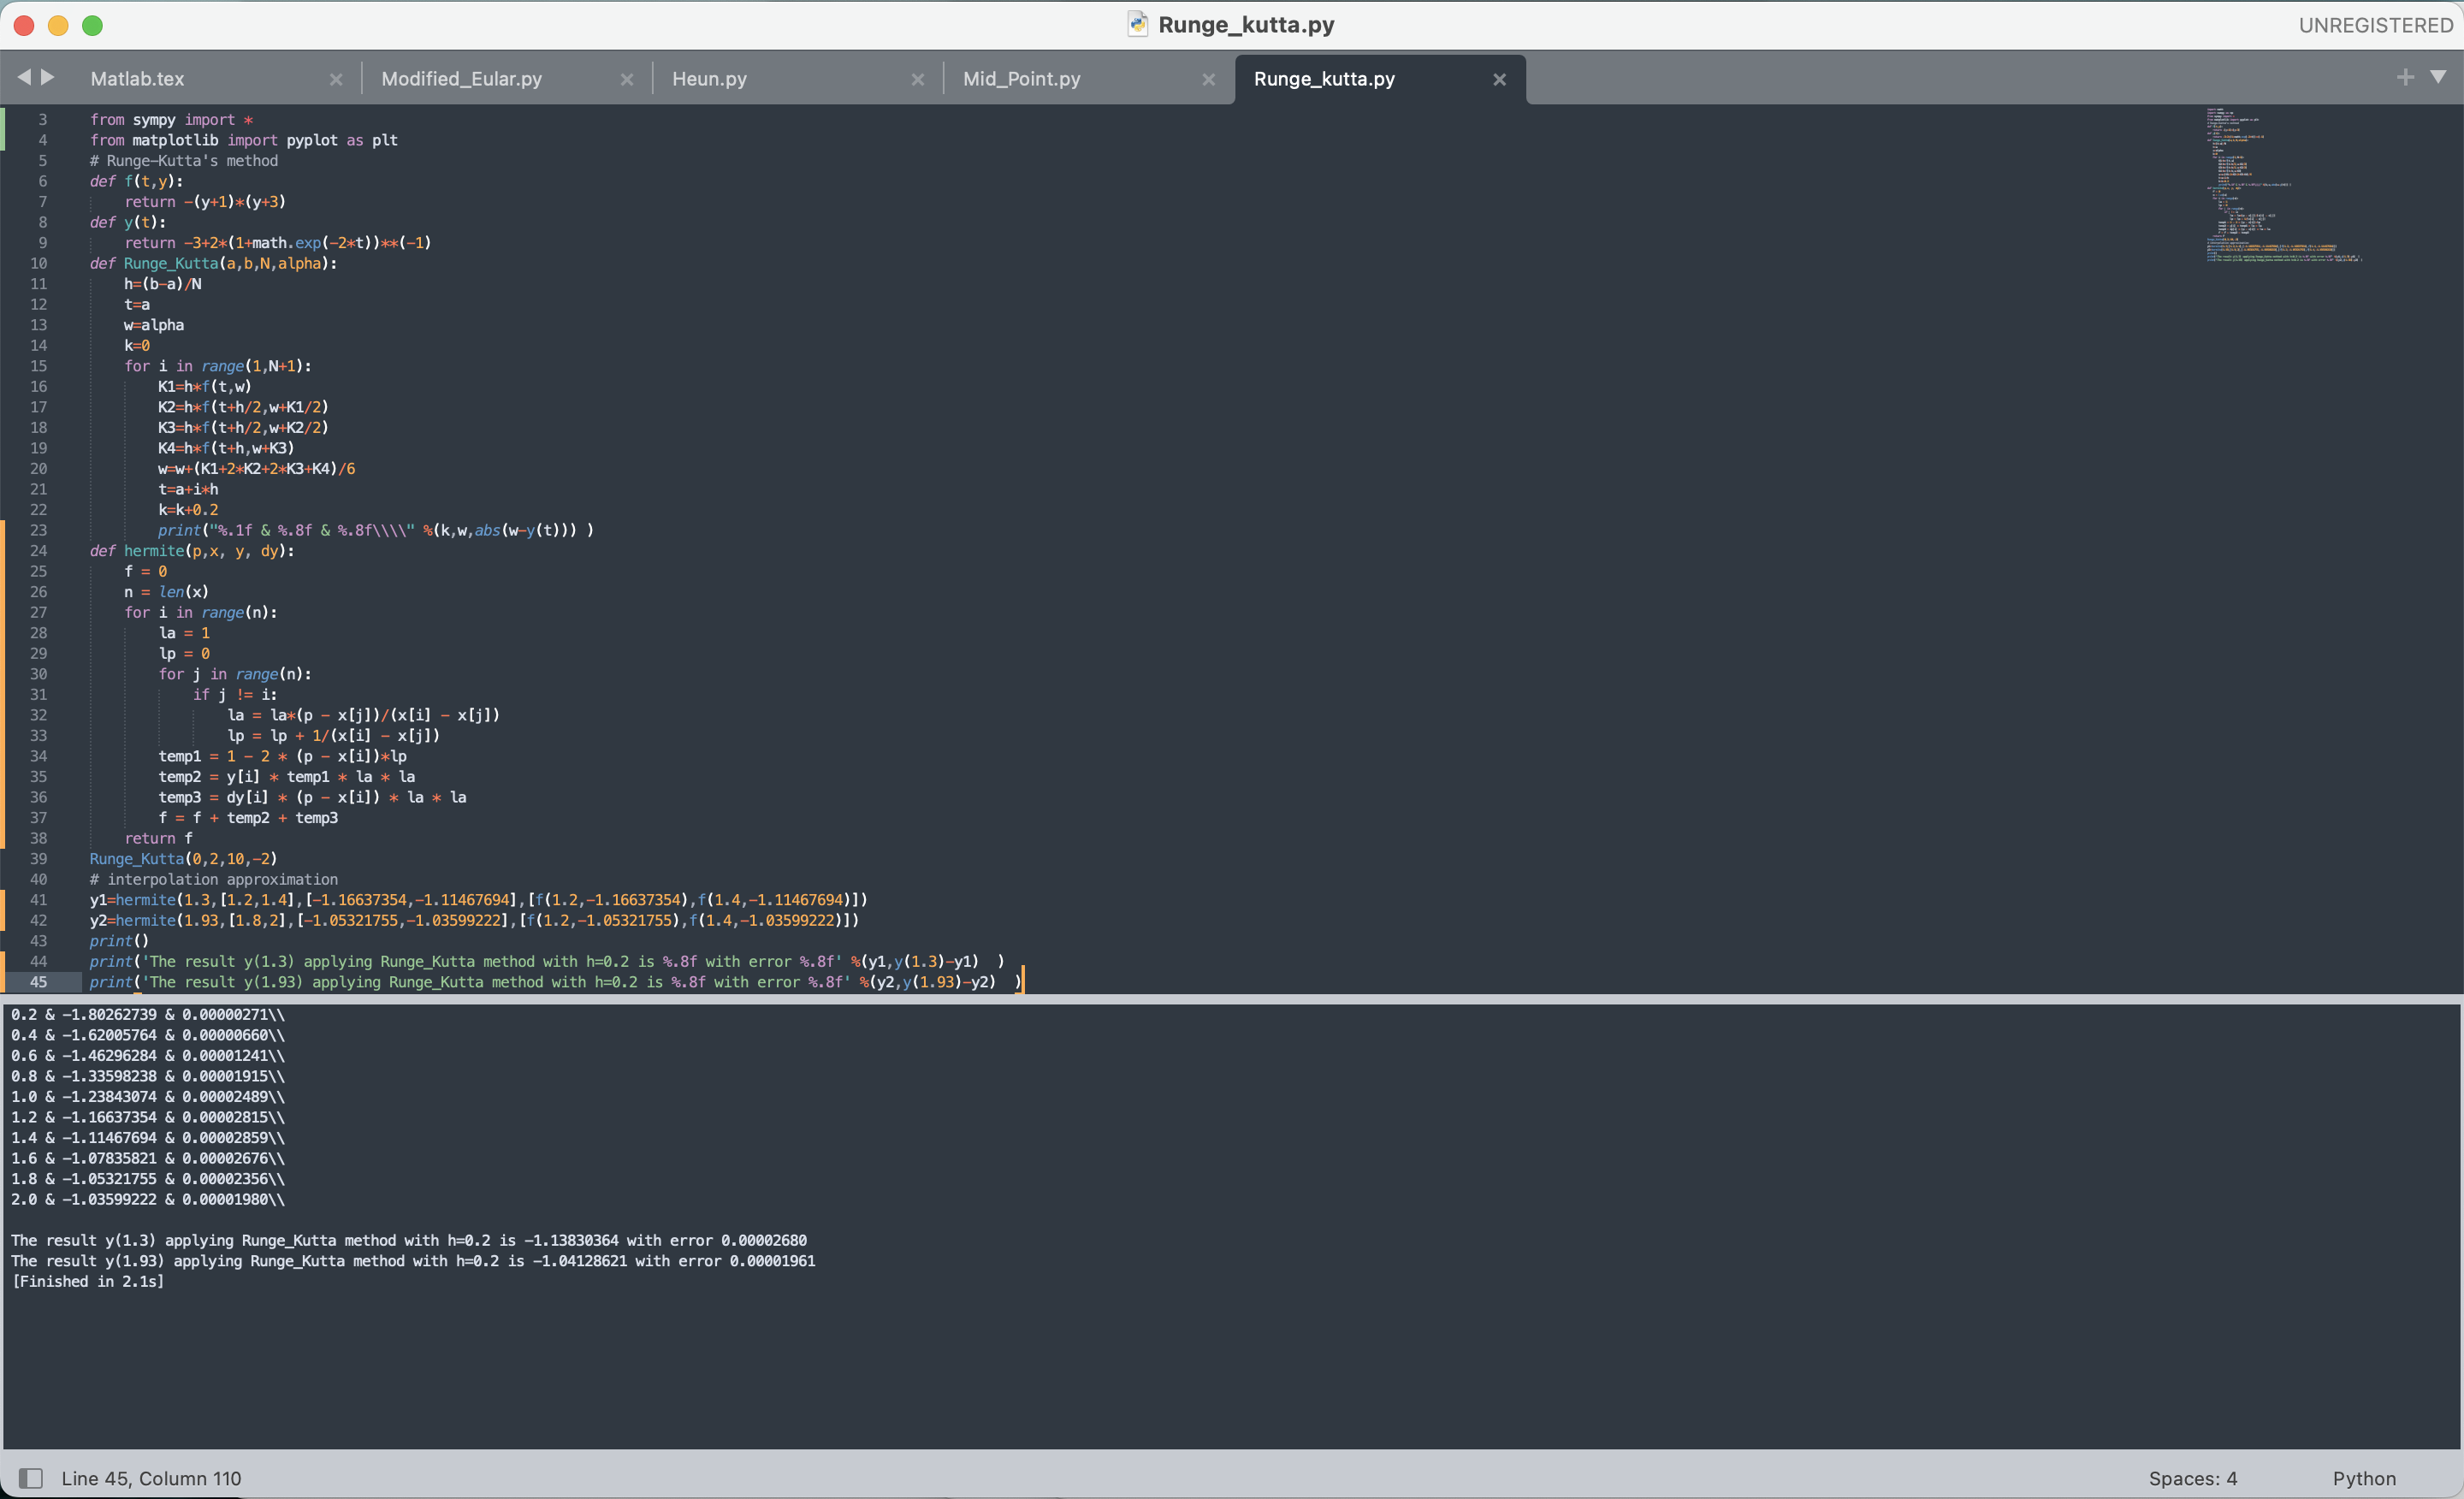
\includegraphics[scale=0.22]{Program4}
    \end{figure}

    And therefore we give a table containing results and errors (reserve nine significant digits): 

    \begin{table}[htbp]
    \centering
    \caption{Results of 5.4/11 (Runge-Kutta's method)}
    \begin{tabular}{c|c|c}
    \toprule
    t& \textbf{Approximation of y(t)} & \textbf{Error} \\ 
    \midrule
    0.2 & -1.80262739 & 0.00000271\\
    0.4 & -1.62005764 & 0.00000660\\
    0.6 & -1.46296284 & 0.00001241\\
    0.8 & -1.33598238 & 0.00001915\\
    1.0 & -1.23843074 & 0.00002489\\
    1.2 & -1.16637354 & 0.00002815\\
    1.4 & -1.11467694 & 0.00002859\\
    1.6 & -1.07835821 & 0.00002676\\
    1.8 & -1.05321755 & 0.00002356\\
    2.0 & -1.03599222 & 0.00001980\\
    \bottomrule
    \end{tabular}
    \end{table}

    Also we find that the error term grows until $t=1.4$, which is contractdict to the earlier claim for Eular's method that the error monotonically increases with t increases. The reason behind this is the same.

    Then for  5.4/12 we use the approximation value of $y(1.2)$,$y(1.4)$,$y'(1.2)$ and $y'(1.4)$ to hermite interpolate $y(1.3)$ as above, which leads to 
    $$ \tilde{y}(1.3)=H_{3}(1.3)=-1.13830364
    $$
    where we denote the approximation value of $y(1.3)$ by $\tilde{y}(1.3)$ and hermite polynomial is being calculated as in the program below
    \begin{python}
    def hermite(p,x, y, dy):
    f = 0
    n = len(x)
    for i in range(n):
        la = 1
        lp = 0
        for j in range(n):
            if j != i:
                la = la*(p - x[j])/(x[i] - x[j])
                lp = lp + 1/(x[i] - x[j])
        temp1 = 1 - 2 * (p - x[i])*lp
        temp2 = y[i] * temp1 * la * la
        temp3 = dy[i] * (p - x[i]) * la * la
        f = f + temp2 + temp3
    return f
    \end{python}
    Similarly, we have $\tilde{y}(1.93)=-1.04128621$. And thus gather the information for the table ( reserve nine significant digits )
    \begin{table}[htbp]
    \centering
    \caption{Results of 5.4/12 (Runge-Kutta's method)}
    \begin{tabular}{c|c|c}
    \toprule
    t& \textbf{Approximation of y(t)} & \textbf{Error} \\ 
    \midrule
    1.3 & -1.13830364 & 0.00002680 \\
    1.93 & -1.04128621 & 0.00001961\\
    \bottomrule
    \end{tabular}
    \end{table}

\subsection{3.5 Conclusion of Above Methods}
    Generally speaking, by comparing the results we see that: 

    1. the Runge-Kutta method gives the best aprroximation but it has the most calculations. 

    2. Heun method gives good approximations near the initial values but gives no approximations further.

    3. Midpoint/Modified-Eular method gives good approximations everywhere and has mild calculations. 

    4. Euler's Method has the smallest calculations but sacrifies its accuracy.

    \textbf{Turn to the next page for section 4.}

\newpage
\section{4. Application of Multistep Method (5.6/3c)}
\subsection{4.1 Program Running and Data Analysis of 5.6/3c }
    We will approximate the solutions to 5.6/3c by applying \textbf{Adams-Bashforth Method}. We run the program as below:

    \begin{figure}[h]
    \centering
    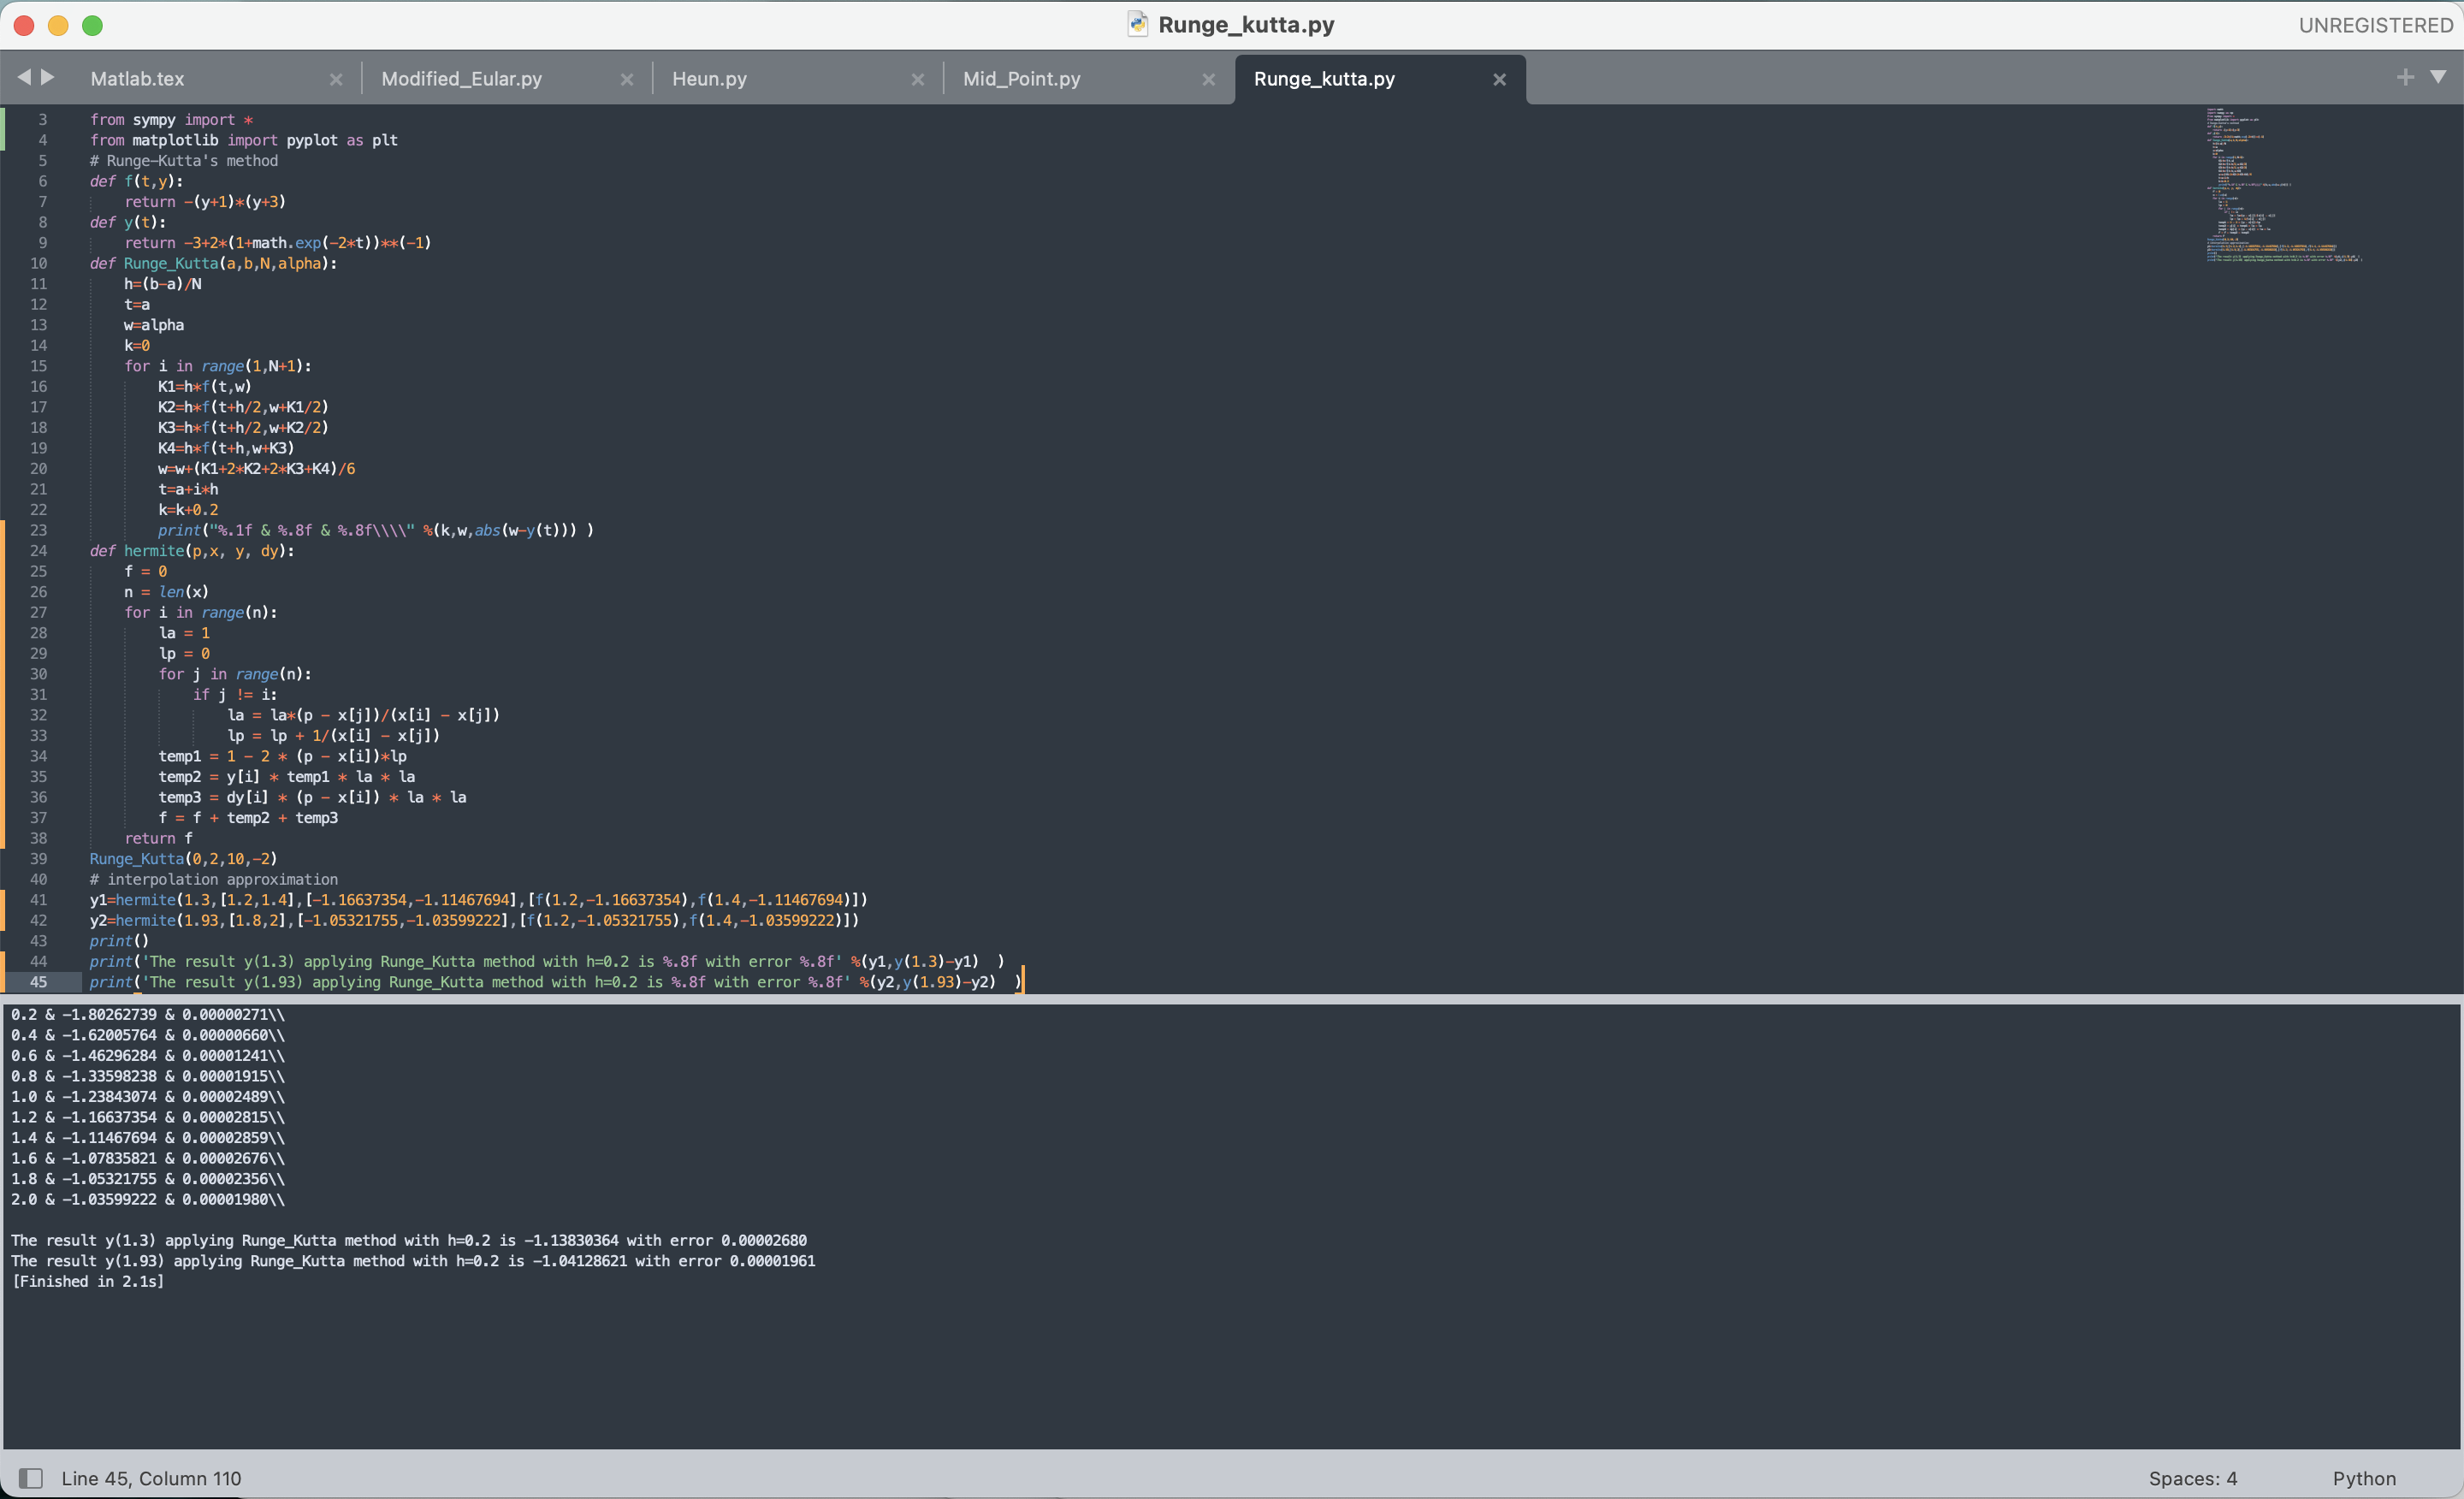
\includegraphics[scale=0.2]{Program4}
    \end{figure}

    Gathering the information, we give the table of results. (reserve nine significant digits)

    \begin{table}[htbp]
    \centering
    \caption{Results of 5.6/3c (Adams-Bashforth method)}
    \begin{tabular}{c|c|c|c|c|c}
    \toprule
    t& \textbf{Real value} & \textbf{2-step} & \textbf{3-step} & \textbf{4-step} & \textbf{5-step}\\ 
    \midrule
    0.1 & -1.90033201 &-1.90033209 &-1.90033209 & -1.90033209 & -1.90033209\\
    0.2 & -1.80262468 &-1.80182214 &-1.80262486 & -1.80262486 & -1.80262486\\
    0.3 & -1.70868739 &-1.70721663 &-1.70876712 & -1.70868768 & -1.70868768\\
    0.4 & -1.62005104 &-1.61811122 &-1.62024327 & -1.62008995 & -1.62005146\\
    0.5 & -1.53788284 &-1.53570097 &-1.53819884 & -1.53793718 & -1.53786761\\
    0.6 & -1.46295043 &-1.46074506 &-1.46337907 & -1.46300534 & -1.46292261\\
    0.7 & -1.39563222 &-1.39358576 &-1.39614605 & -1.39567144 & -1.39559281\\
    0.8 & -1.33596323 &-1.33420670 &-1.33652621 & -1.33597925 & -1.33592042\\
    0.9 & -1.28370213 &-1.28231190 &-1.28427720 & -1.28369238 & -1.28365952\\
    1.0 & -1.23840584 &-1.23740929 &-1.23896052 & -1.23837336 & -1.23836930\\
    1.1 & -1.19950098 &-1.19888717 &-1.20001057 & -1.19945122 & -1.19947117\\
    1.2 & -1.16634539 &-1.16607721 &-1.16679398 & -1.16628513 & -1.16632443\\
    1.3 & -1.13827684 &-1.13830220 &-1.13865663 & -1.13821228 & -1.13826257\\
    1.4 & -1.11464835 &-1.11490931 &-1.11495817 & -1.11458465 & -1.11464097\\
    1.5 & -1.09485175 &-1.09529098 &-1.09509518 & -1.09479250 & -1.09484815\\
    1.6 & -1.07833145 &-1.07889647 &-1.07851510 & -1.07827891 & -1.07833179\\
    1.7 & -1.06459093 &-1.06523630 &-1.06472296 & -1.06454612 & -1.06459229\\
    1.8 & -1.05319399 &-1.05388219 &-1.05328300 & -1.05315708 & -1.05319726\\
    1.9 & -1.04376254 &-1.04446387 &-1.04381686 & -1.04373311 & -1.04376513\\
    \bottomrule
    \end{tabular}
    \end{table}

    Comparing the results with the real values we find that with the steps increase, the more accurate the Adams-Bashforth method become. (Accuracy is measured by the difference between real value and approximation value.)

\subsection{4.2 Program Running and Data Analysis of 5.6/5,6 }
    We will approximate the solutions to 5.6/3c by applying \textbf{Adams Fourth-Order Predictor-Corrector Method}. We run the program as below:
    \begin{figure}[h]
    \centering
    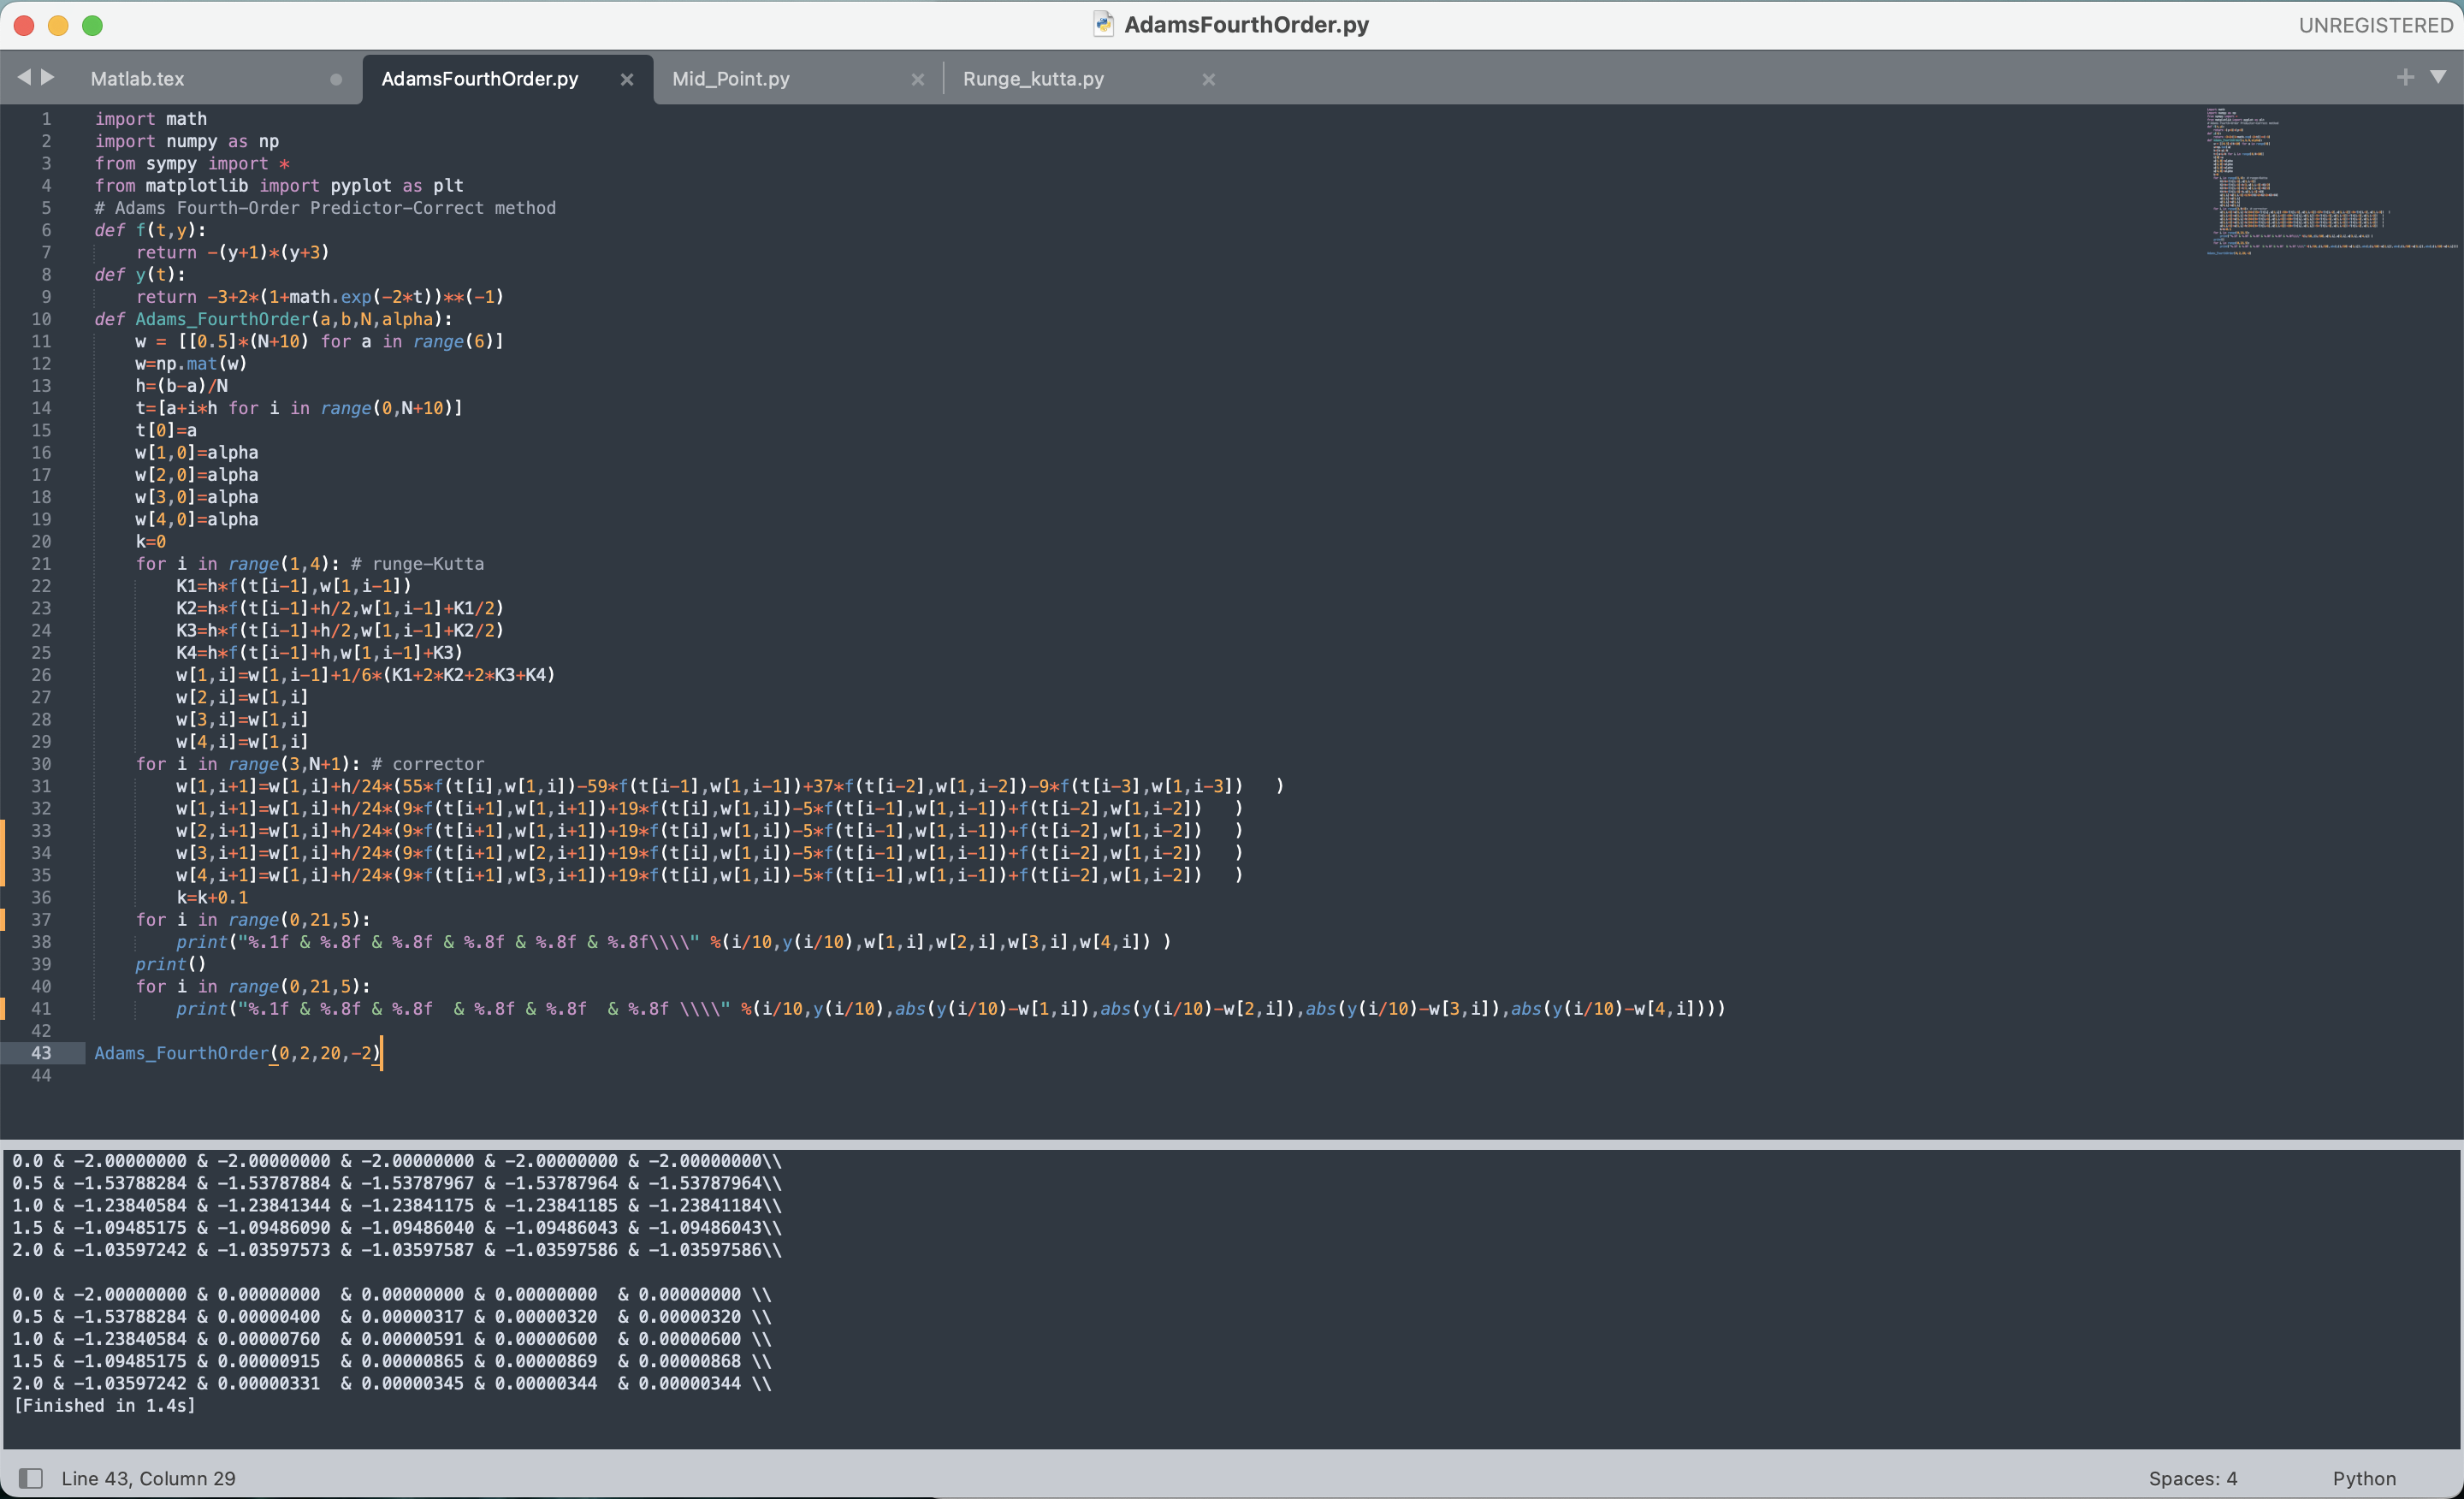
\includegraphics[scale=0.2]{Program5}
    \end{figure}

    In which we change the algorithm (iterate the formula in the algorithm) so that it can make the corrector be iterated for p iterations. (p=2,3,4)

    And we shall gather the results in a table as below

    \begin{table}[htbp]
    \centering
    \caption{Results of 5.6/5,6 (Adams Fourth-Order Predictor-Corrector Method)}
    \begin{tabular}{c|c|c|c|c|c}
    \toprule
    t& \textbf{Real value} & \textbf{1-iteration} & \textbf{2-iteration} & \textbf{3-iteration} & \textbf{4-iteration}\\ 
    \midrule
    0.0 & -2.00000000 &-2.00000000 &-2.00000000 & -2.00000000 & -2.00000000\\
    0.5 & -1.53788284 &-1.53787884 &-1.53787967 & -1.53787964 & -1.53787964\\
    1.0 & -1.23840584 &-1.23841344 &-1.23841175 & -1.23841185 & -1.23841184\\
    1.5 & -1.09485175 &-1.09486090 &-1.09486040 & -1.09486043 & -1.09486043\\
    2.0 & -1.03597242 &-1.03597573 &-1.03597587 & -1.03597586 & -1.03597586\\
    \bottomrule
    \end{tabular}
    \end{table}

    and with the errors also calculated in the table below.

    \begin{table}[htbp]
    \centering
    \caption{Results of 5.6/5,6 (Adams Fourth-Order Predictor-Corrector Method)}
    \begin{tabular}{c|c|c|c|c}
    \toprule
    t & \textbf{Errors of 1-iteration} & \textbf{Errors of 2-iteration} & \textbf{Errors of 3-iteration} & \textbf{Errors of 4-iteration}\\ 
    \midrule
    0.0 & 0.00000000  & 0.00000000 & 0.00000000  & 0.00000000 \\
    0.5 & 0.00000400  & 0.00000317 & 0.00000320  & 0.00000320 \\
    1.0 & 0.00000760  & 0.00000591 & 0.00000600  & 0.00000600 \\
    1.5 & 0.00000915  & 0.00000865 & 0.00000869  & 0.00000868 \\
    2.0 & 0.00000331  & 0.00000345 & 0.00000344  & 0.00000344 \\
    \bottomrule
    \end{tabular}
    \end{table}

    From the above table 12 we find that for almost all values of t, the best approximation is given by 2-iteration. So the best p is 2. 


\newpage
\subsection{5 Application Runge-Kutta for Systems Algorithms (5.9/2c)}
    \subsection{5.1 Program Running and Data Analysis of 5.9/2c (Runge-Kutta for Systems Algorithms)}
    We will approximate the solutions to 5.9/2c by applying \textbf{Runge-Kutta Method for Systems of Differential Equations}. First observe in chapter 5.9 we can only deal with the numerical approximation of the m-th order system in the form of (5.44). But in 5.9/2c, we will approximate the solutions of

    $$y'''+2y''-y'-2y=e^t    
    $$

    s.t. the initial conditions: $y(0)=1,y'(0)=2,y''(0)=0$.


    As a result of the above argument we can't directly apply the algorithm. But if we first magically suppose
    $$ y_1:=y \quad y_2:=y' \quad y_3:=y''
    $$
    Then the form of 5.9/2c will be transformed to
    \begin{equation}
    \left\{
    \begin{aligned}
    y_{1}'&=y_2\\
    y_{2}'&=y_3\\ 
    y_{3}'&=2y_{1}+y_{2}-2y_{3}+e^{t}\\  
    \end{aligned}
    \right.
    \end{equation}

    s.t. the initial conditions: $y_{1}(0)=1,y_{2}(0)=2,y_{3}(0)=0$. 

    First and foremost, we run the program as below (Meanwhile we also display the running time as a byproduct.)

    \begin{figure}[h]
    \centering
    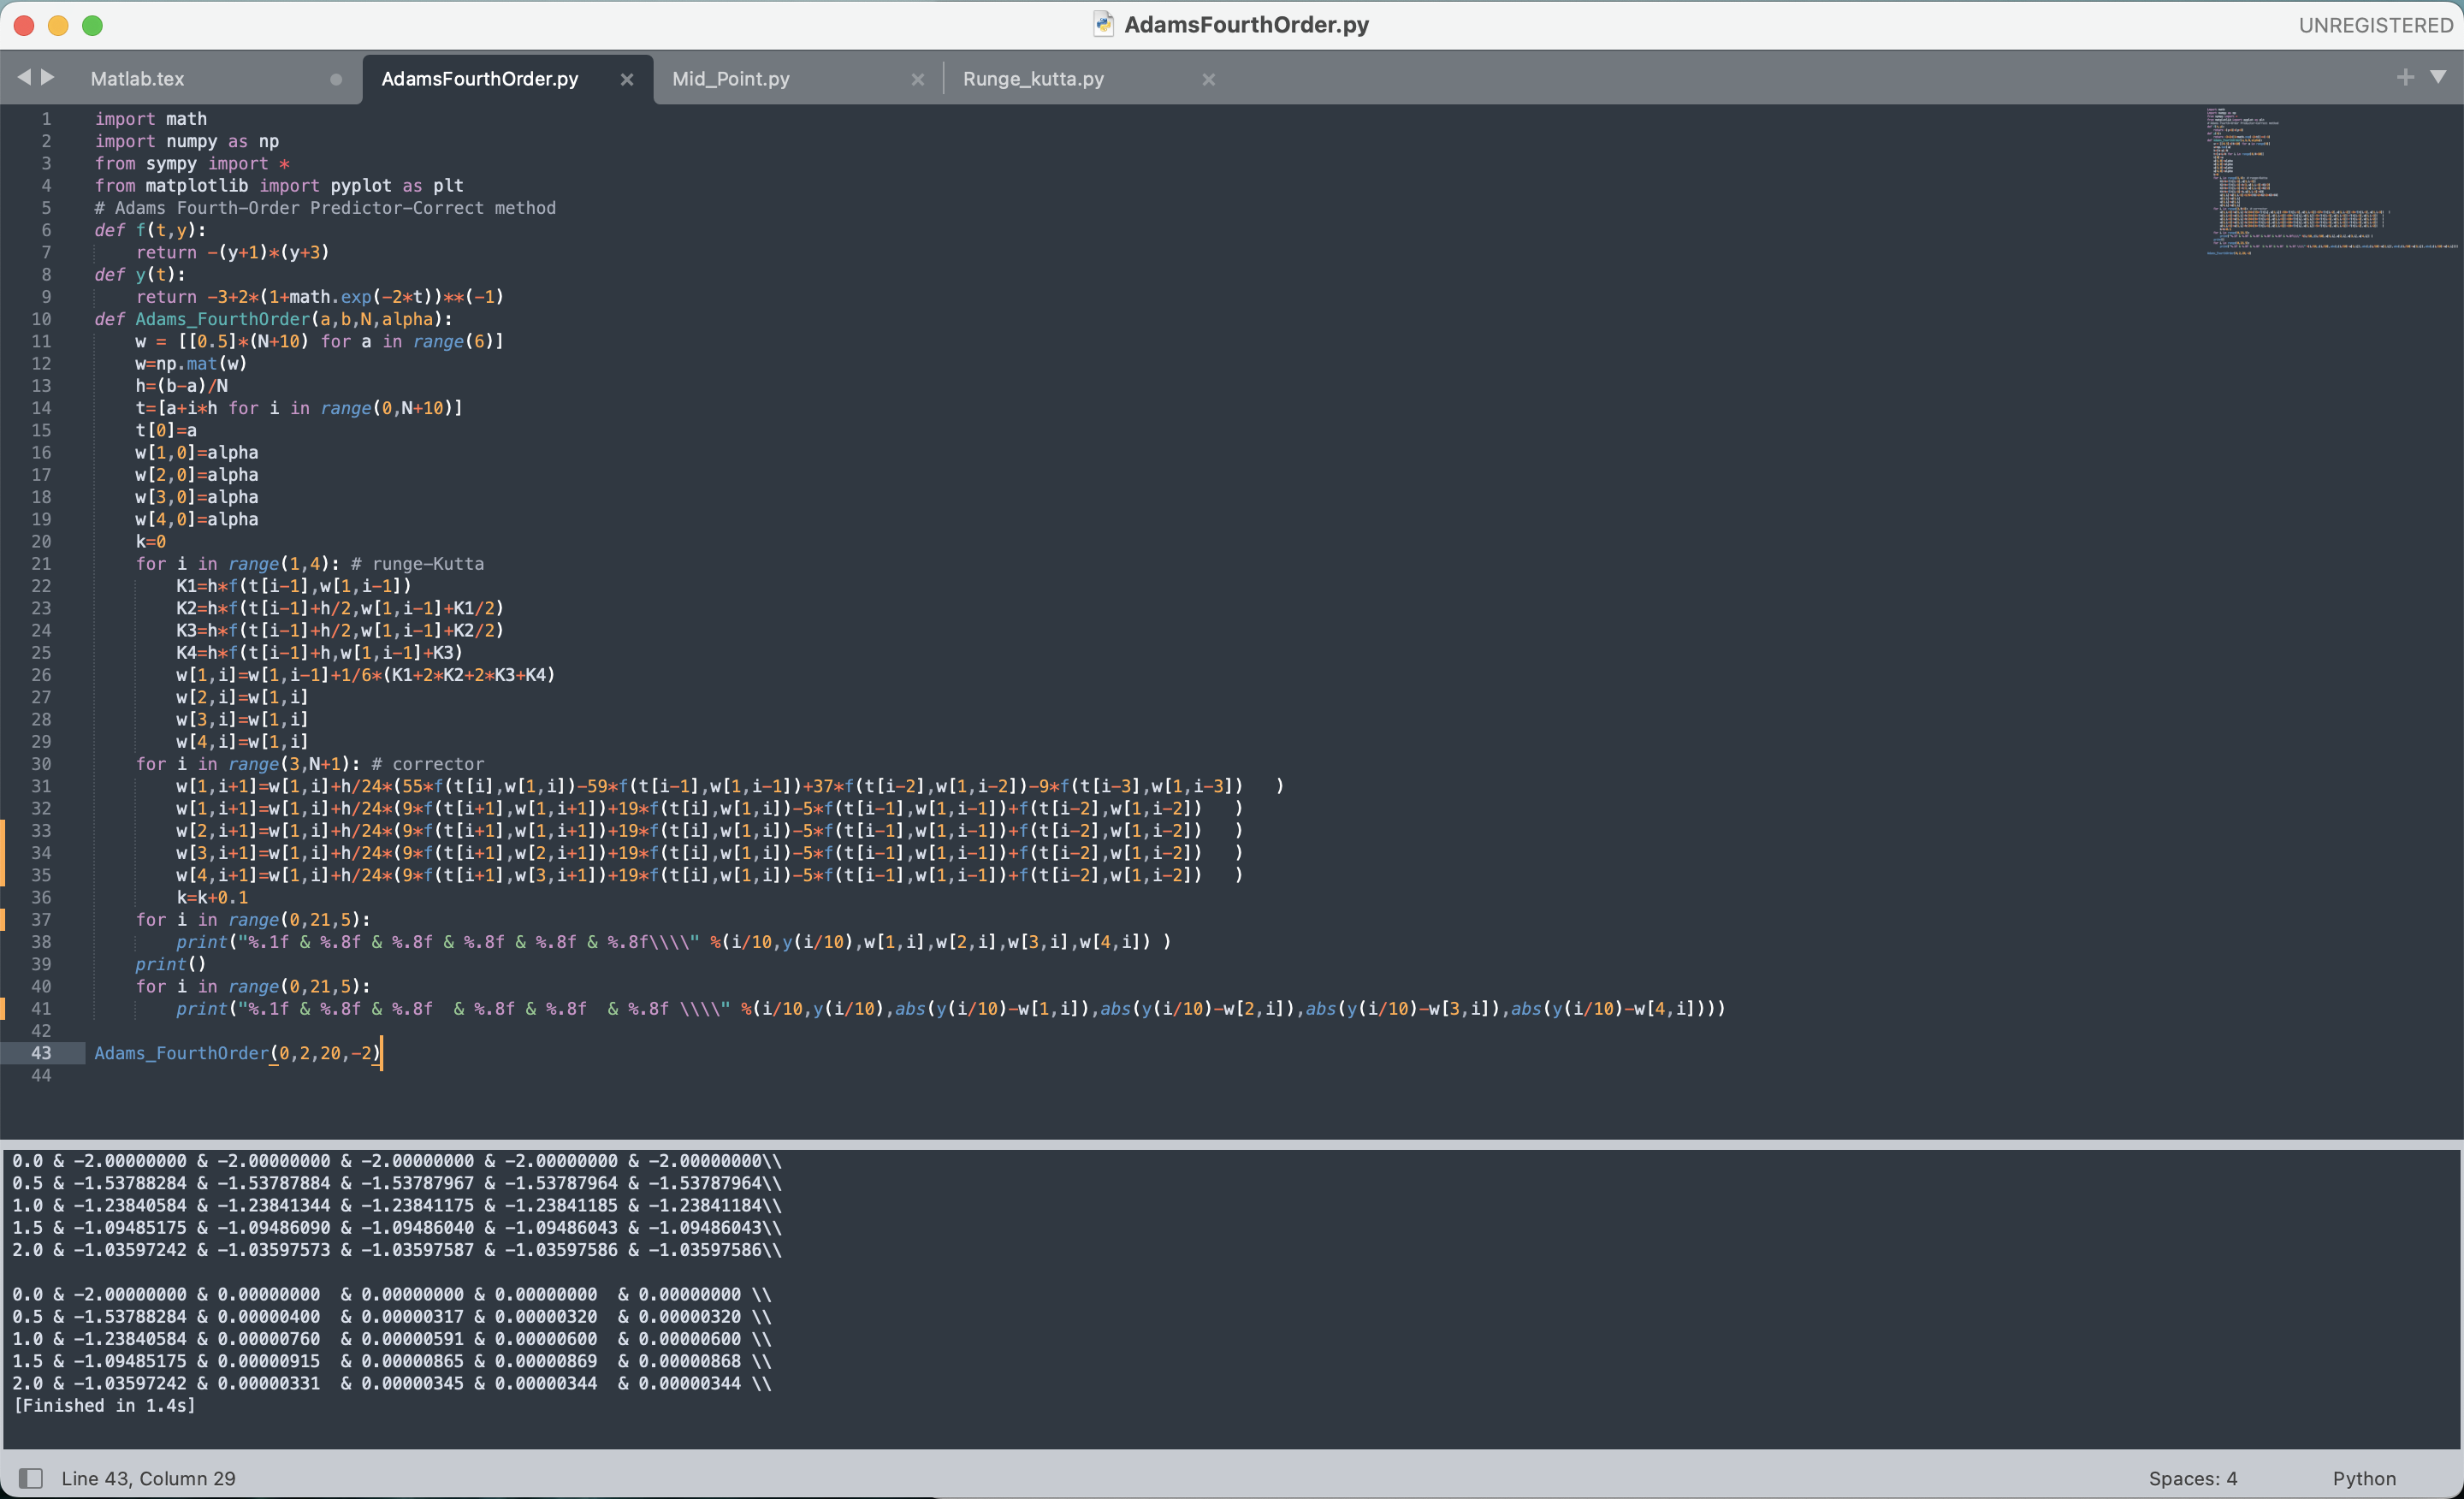
\includegraphics[scale=0.2]{Program5}
    \end{figure}

    We see that approximated values of $y(t)$, $y'(t)$ and $y''(t)$ are all showed in the display table separated by $\&$ and $\backslash\backslash$ finished in $2.0s$. And the errors represent the difference between real values of $y(t)$ and approximation values of $y(t)$ in a step of $h=0.2$ as requested by the question text.

    And therefore we shall gather the results into the table below which can represent the results more clearly, where we \textbf{reserve nine significant digits}.

    Observe that the error accumulates with t grows as usual. But as a windfall we can approximate the solutions of $y'(t)$ and $y''(t)$. Still the details are gathered in the table below.

    \begin{table}[t]
    \centering
    \caption{Results of 5.9/2c (Adams Fourth-Order Predictor-Corrector Method)}
    \begin{tabular}{c|c|c|c|c|c}
    \toprule
    t& \textbf{Real value} & \textbf{Approximation of $y(t)$} & \textbf{Error} & \textbf{Approximation of $y'(t)$} & \textbf{Approximation of $y''(t)$}\\ 
    \midrule
    0.0 & 1.00000000 & 1.00000000 & 0.00000000 & 2.00000000 & 0.00000000\\
    0.2 & 1.40637383 & 1.40633678 & 0.00003705 & 2.09439538 & 0.91961556\\
    0.4 & 1.84923495 & 1.84918146 & 0.00005350 & 2.36188926 & 1.74722932\\
    0.6 & 2.36197037 & 2.36190903 & 0.00006134 & 2.79290064 & 2.56757686\\
    0.8 & 2.97762424 & 2.97755643 & 0.00006781 & 3.39310710 & 3.45012070\\
    1.0 & 3.73170445 & 3.73162695 & 0.00007749 & 4.18124911 & 4.45721868\\
    1.2 & 4.66469806 & 4.66460440 & 0.00009366 & 5.18835555 & 5.65033178\\
    1.4 & 5.82454694 & 5.82442783 & 0.00011912 & 6.45808521 & 7.09509448\\
    1.6 & 7.26928830 & 7.26913151 & 0.00015679 & 8.04801932 & 8.86584062\\
    1.8 & 9.07004289 & 9.06983275 & 0.00021014 & 10.03184298 & 11.05003348\\
    2.0 & 11.31452924 & 11.31424573 & 0.00028351 & 12.50243368 & 13.75296416\\
    2.2 & 14.11129305 & 14.11091055 & 0.00038250 & 15.57594327 & 17.10304019\\
    2.4 & 17.59486416 & 17.59434982 & 0.00051435 & 19.39702265 & 21.25797699\\
    2.6 & 21.93209017 & 21.93140177 & 0.00068840 & 24.14540203 & 26.41222100\\
    2.8 & 27.32994449 & 27.32902779 & 0.00091670 & 30.04410928 & 32.80597197\\
    3.0 & 34.04517155 & 34.04395688 & 0.00121468 & 37.36968748 & 40.73623289\\
    \bottomrule
    \end{tabular}
    \end{table}
\newpage
\section{6. Code Appendix}
    \subsection{6.1 Eular's Method}
    \begin{python}
    import math
    Real=math.exp(-5)+5
    # eular's method
    def f(t,y):
        return -y+t+1
    def eular(a,b,N,alpha):
        h=(b-a)/N
        t=a
        w=alpha
        for i in range(1,N+1):
            w=w+h*f(t,w)
            t=a+i*h
        return w
    print('The result applying Eular method with h=0.2 is',eular(0,5,25,1),'with error',Real-eular(0,5,25,1))
    print('The result applying Eular method with h=0.1 is',eular(0,5,50,1),'with error',Real-eular(0,5,50,1))
    print('The result applying Eular method with h=0.05 is',eular(0,5,100,1),'with error',Real-eular(0,5,100,1))
    print('The result applying Eular method with h=0.0014 is',eular(0,5,3535,1),'with error',Real-eular(0,5,3535,1))
    \end{python}

\subsection{6.2 Modified Eular's Method}   
\begin{python}
import math
# Modified_Eular's method
def f(t,y):
    return -(y+1)*(y+3)
def y(t):
    return -3+2*(1+math.exp(-2*t))**(-1)
def Modified_Eular(a,b,N,alpha):
    h=(b-a)/N
    t=a
    w=alpha
    k=0
    for i in range(1,N+1):
        w=w+h/2*(f(t,w)+f(t+h,w+h*f(t,w)))
        t=a+i*h
        k=k+0.2
        print("%.1f & %.8f & %.8f\\\\" %(k,w,y(t)-w) )
def interpolation(t,a,b,c,d):
    return (d-c)/(b-a)*(t-a)+c
Modified_Eular(0,2,10,-2)
# interpolation approximation 
y1=interpolation(1.3,1.2,1.4,-1.172210612839059,-1.1200763302151344)
y2=interpolation(1.93,1.8,2,-1.0571698907180425,-1.0391938189655483)
print()
print('The result y(1.3) applying Modified_Eular method with h=0.2 is %.8f with error %.8f' %(y1,y(1.3)-y1)  )
print('The result y(1.93) applying Modified_Eular method with h=0.2 is%.8f with error %.8f' %(y2,y(1.93)-y2)  )
\end{python}

\subsection{6.3 Modified Eular's Method} 
\begin{python}
import math
# Heun's method
def f(t,y):
    return -(y+1)*(y+3)
def y(t):
    return -3+2*(1+math.exp(-2*t))**(-1)
def Heun(a,b,N,alpha):
    h=(b-a)/N
    t=a
    w=alpha
    k=0
    for i in range(1,N+1):
        w=w+h/4*(f(t,w)+3*f(t+2/3*h,w+2/3*h*f(t,w)))
        t=a+i*h
        k=k+0.2
        print("%.1f & %.8f & %.8f\\\\" %(k,w,abs(w-y(t))) )
def interpolation(t,a,b,c,d):
    return (d-c)/(b-a)*(t-a)+c
Heun(0,2,10,-2)
# interpolation approximation 
y1=interpolation(1.3,1.2,1.4,-1.1699932308872074,-1.1183617793290332)
y2=interpolation(1.93,1.8,2,-1.0562505811390515,-1.0391938189655483)
print()
print('The result y(1.3) applying Heun method with h=0.2 is %.8f with error %.8f' %(y1,y(1.3)-y1)  )
print('The result y(1.93) applying Heun method with h=0.2 is %.8f with error %.8f' %(y2,y(1.93)-y2)  )
\end{python}

\subsection{6.4 Heun's Method}
\begin{python}
import math
# Mid_Point method
def f(t,y):
    return -(y+1)*(y+3)
def y(t):
    return -3+2*(1+math.exp(-2*t))**(-1)
def Mid_Point(a,b,N,alpha):
    h=(b-a)/N
    t=a
    w=alpha
    k=0
    for i in range(1,N+1):
        w=w+h*f(t+h/2,w+h/2*f(t,w))
        t=a+i*h
        k=k+0.2
        print("%.1f & %.8f & %.8f\\\\" %(k,w,abs(w-y(t))) )
def interpolation(t,a,b,c,d):
    return (d-c)/(b-a)*(t-a)+c
Mid_Point(0,2,10,-2)
# interpolation approximation 
y1=interpolation(1.3,1.2,1.4,-1.1688975879735313,-1.1175164873711958)
y2=interpolation(1.93,1.8,2,-1.0557987215668139,-1.038222697151529)
print()
print('The result y(1.3) applying Mid_Point method with h=0.2 is %.8f with error %.8f' %(y1,y(1.3)-y1)  )
print('The result y(1.93) applying Mid_Point method with h=0.2 is %.8f with error %.8f' %(y2,y(1.93)-y2)  )  
\end{python}

\subsection{6.5 Midpoint Method}
\begin{python}
import math
# Mid_Point method
def f(t,y):
    return -(y+1)*(y+3)
def y(t):
    return -3+2*(1+math.exp(-2*t))**(-1)
def Mid_Point(a,b,N,alpha):
    h=(b-a)/N
    t=a
    w=alpha
    k=0
    for i in range(1,N+1):
        w=w+h*f(t+h/2,w+h/2*f(t,w))
        t=a+i*h
        k=k+0.2
        print("%.1f & %.8f & %.8f\\\\" %(k,w,abs(w-y(t))) )
def interpolation(t,a,b,c,d):
    return (d-c)/(b-a)*(t-a)+c
Mid_Point(0,2,10,-2)
# interpolation approximation 
y1=interpolation(1.3,1.2,1.4,-1.1688975879735313,-1.1175164873711958)
y2=interpolation(1.93,1.8,2,-1.0557987215668139,-1.038222697151529)
print()
print('The result y(1.3) applying Mid_Point method with h=0.2 is %.8f with error %.8f' %(y1,y(1.3)-y1)  )
print('The result y(1.93) applying Mid_Point method with h=0.2 is %.8f with error %.8f' %(y2,y(1.93)-y2)  )
\end{python}

\subsection{6.6 Runge-Kutta's Method}
\begin{python}
import math
import numpy as np
from sympy import *
from matplotlib import pyplot as plt
# Runge-Kutta's method
def f(t,y):
    return -(y+1)*(y+3)
def y(t):
    return -3+2*(1+math.exp(-2*t))**(-1)
def Runge_Kutta(a,b,N,alpha):
    h=(b-a)/N
    t=a
    w=alpha
    k=0
    for i in range(1,N+1):
        K1=h*f(t,w)
        K2=h*f(t+h/2,w+K1/2)
        K3=h*f(t+h/2,w+K2/2)
        K4=h*f(t+h,w+K3)
        w=w+(K1+2*K2+2*K3+K4)/6
        t=a+i*h
        k=k+0.2
        print("%.1f & %.8f & %.8f\\\\" %(k,w,abs(w-y(t))) )
def hermite(p,x, y, dy):
    f = 0
    n = len(x)
    for i in range(n):
        la = 1
        lp = 0
        for j in range(n):
            if j != i:
                la = la*(p - x[j])/(x[i] - x[j])
                lp = lp + 1/(x[i] - x[j])
        temp1 = 1 - 2 * (p - x[i])*lp
        temp2 = y[i] * temp1 * la * la
        temp3 = dy[i] * (p - x[i]) * la * la
        f = f + temp2 + temp3
    return f
Runge_Kutta(0,2,20,-2)
# interpolation approximation 
y1=hermite(1.3,[1.2,1.4],[-1.16637354,-1.11467694],[f(1.2,-1.16637354),f(1.4,-1.11467694)])
y2=hermite(1.93,[1.8,2],[-1.05321755,-1.03599222],[f(1.2,-1.05321755),f(1.4,-1.03599222)])
print()
print('The result y(1.3) applying Runge_Kutta method with h=0.2 is %.8f with error %.8f' %(y1,y(1.3)-y1)  )
print('The result y(1.93) applying Runge_Kutta method with h=0.2 is %.8f with error %.8f' %(y2,y(1.93)-y2)  )ult y(1.93) applying Mid_Point method with h=0.2 is %.8f with error %.8f' %(y2,y(1.93)-y2)  )
\end{python}

\subsection{6.7 Adams Bashforth's method}
\begin{python}
import math
import numpy as np
from sympy import *
from matplotlib import pyplot as plt
# Adams_Bashforth's method
def f(t,y):
    return -(y+1)*(y+3)
def y(t):
    return -3+2*(1+math.exp(-2*t))**(-1)
def Adams_Bashforth(a,b,N,alpha):
    w = [[0.5]*(N+10) for a in range(6)]
    w=np.mat(w)
    h=(b-a)/N
    t=a
    w[2,0]=alpha
    w[2,1]=-1.90033209
    w[3,0]=alpha
    w[3,1]=-1.90033209
    w[3,2]=-1.80262486
    w[4,0]=alpha
    w[4,1]=-1.90033209
    w[4,2]=-1.80262486
    w[4,3]=-1.70868768 
    w[5,0]=alpha
    w[5,1]=-1.90033209
    w[5,2]=-1.80262486
    w[5,3]=-1.70868768 
    w[5,4]=-1.62005146
    k=0
    for i in range(1,N):
        w[2,i+1]=w[2,i]+h/2*(3*f(t,w[2,i])-f(t-h,w[2,i-1]) )
        w[3,i+2]=w[3,i+1]+h/12*(23*f(t,w[3,i+1])-16*f(t-h,w[3,i])+5*f(t-2*h,w[3,i-1]) )
        w[4,i+3]=w[4,i+2]+h/24*(55*f(t,w[4,i+2])-59*f(t-h,w[4,i+1])
        +37*f(t-2*h,w[4,i])-9*f(t-3*h,w[4,i-1]) )
        w[5,i+4]=w[5,i+3]+h/720*(1901*f(t,w[5,i+3])-2774*f(t-h,w[5,i+2])
        +2616*f(t-2*h,w[5,i+1])-1274*f(t-3*h,w[5,i])+251*f(t-4*h,w[5,i-1]))
        t=a+i*h
        k=k+0.1
        print("%.1f & %.8f &%.8f &%.8f & %.8f & %.8f\\\\" %(k,y(k),w[2,i],w[3,i],w[4,i],w[5,i]) )
Adams_Bashforth(0,2,20,-2)
\end{python}

\subsection{6.8 Runge-Kutta Method for Systems of Differential Equations}
\begin{python}
import math
import numpy as np
from sympy import *
from matplotlib import pyplot as plt
# initialization
w=[0.5,0.5,0.5,0.5]
k=[[0.5]*5 for i in '12345']
k=np.matrix(k)
def y(t):
    return 43/36*math.exp(t)+1/4*math.exp(-t)-4/9*math.exp(-2*t)+1/6*t*math.exp(t)
def f1(t,w1,w2,w3):
    return w2
def f2(t,w1,w2,w3):
    return w3
def f3(t,w1,w2,w3):
    return 2*w1+w2-2*w3+math.exp(t)
# Runge-Kutta Method for Systems of Differential Equations
def Runge_Kutta_Systems(a,b,N,alpha):
    h=(b-a)/N 
    t=a
    for j in range(1,4):
        w[j]=alpha[j]
    print("%.1f & %.8f & %.8f & %.8f & %.8f & %.8f\\\\" %(t,y(t),w[1],abs(y(t)-w[1]),w[2],w[3]) )
    for i in range(1,N+1):
        # 1
        k[1,1]=h*f1(t,w[1],w[2],w[3])
        k[1,2]=h*f2(t,w[1],w[2],w[3])
        k[1,3]=h*f3(t,w[1],w[2],w[3])
        # 2
        k[2,1]=h*f1(t+h/2,w[1]+k[1,1]/2,w[2]+k[1,2]/2,w[3]+k[1,3]/2)
        k[2,2]=h*f2(t+h/2,w[1]+k[1,1]/2,w[2]+k[1,2]/2,w[3]+k[1,3]/2)
        k[2,3]=h*f3(t+h/2,w[1]+k[1,1]/2,w[2]+k[1,2]/2,w[3]+k[1,3]/2)
        # 3
        k[3,1]=h*f1(t+h/2,w[1]+k[2,1]/2,w[2]+k[2,2]/2,w[3]+k[2,3]/2)
        k[3,2]=h*f2(t+h/2,w[1]+k[2,1]/2,w[2]+k[2,2]/2,w[3]+k[2,3]/2)
        k[3,3]=h*f3(t+h/2,w[1]+k[2,1]/2,w[2]+k[2,2]/2,w[3]+k[2,3]/2)
        # 4
        k[4,1]=h*f1(t+h,w[1]+k[3,1],w[2]+k[3,2],w[3]+k[3,3])
        k[4,2]=h*f2(t+h,w[1]+k[3,1],w[2]+k[3,2],w[3]+k[3,3])
        k[4,3]=h*f3(t+h,w[1]+k[3,1],w[2]+k[3,2],w[3]+k[3,3])
        for j in range(1,4):
            w[j]=w[j]+(k[1,j]+2*k[2,j]+2*k[3,j]+k[4,j])/6
        t=a+i*h 
        print("%.1f & %.8f & %.8f & %.8f & %.8f & %.8f\\\\" %(t,y(t),w[1],abs(y(t)-w[1]),w[2],w[3]) )
Runge_Kutta_Systems(0,3,15,[0,1,2,0])
\end{python}

   
\end{document}
